\documentclass[12pt, twoside]{report}

\usepackage[utf8]{inputenc}
\usepackage{graphicx}
\graphicspath{{images/}}
\usepackage[a4paper,width=150mm,top=25mm,bottom=25mm,bindingoffset=6mm]{geometry}
\usepackage{fancyhdr}
\pagestyle{fancy}

%\usepackage[style=alphabetic, sorting=none]{biblatex}
%\addbibresource{references.bib}


\usepackage{pdfpages}

\title{Automated collection of multi-source spatial information for emergency management}
\author{Sandra Moen}
\date{Spring 2018}
\begin{document}

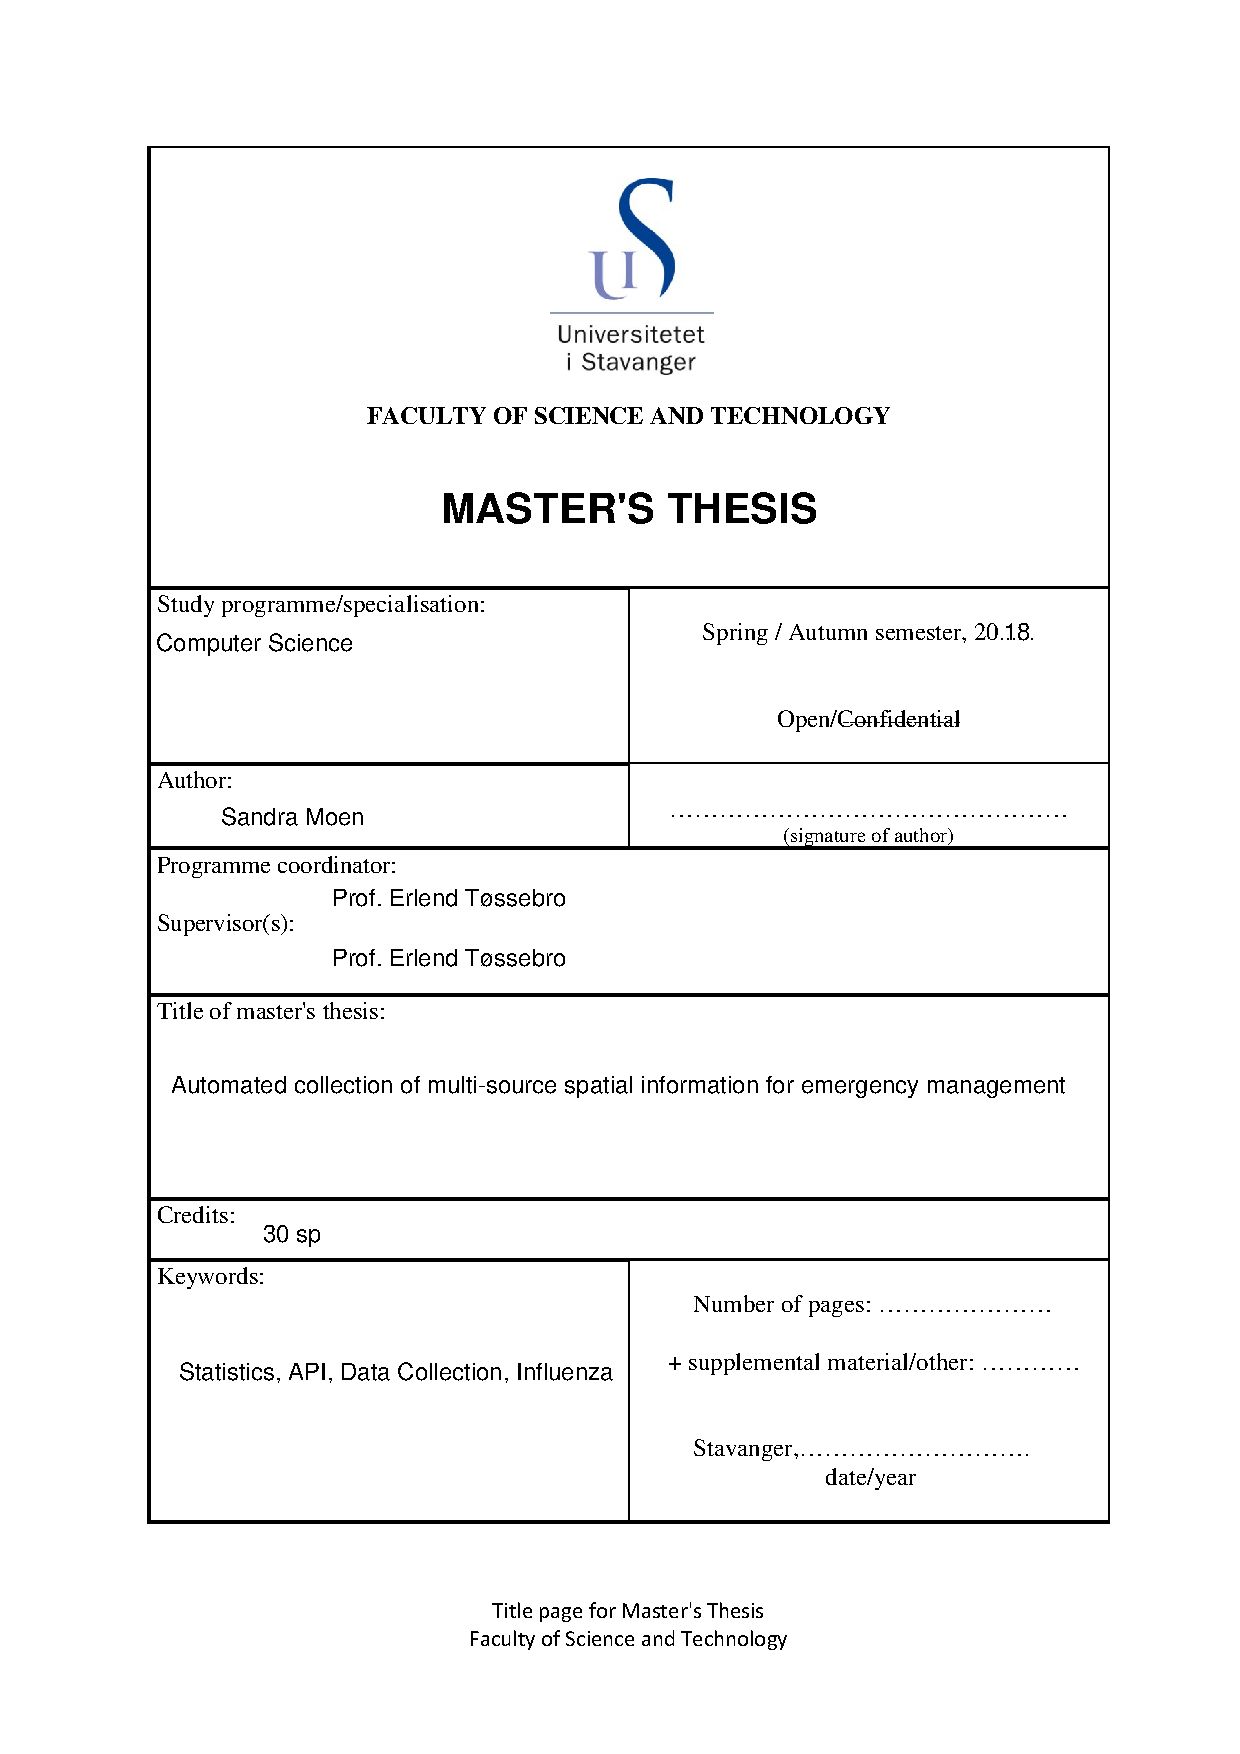
\includepdf[pages=-]{englishFrontPageUiS_WIP.pdf}

\begin{titlepage}
	\begin{center}
		\vspace*{1cm}
		
		\Huge
		\textbf{Automated collection of multi-source spatial information for emergency management}
		
		\vspace{0.5cm}
		\LARGE
		Tracking the influenza seasons
		
		\vspace{1.5cm}
		
		\textbf{Sandra Moen}
		
		\vfill
		
		A thesis presented for the degree of \\
		Master of Science in Computer Science
		
		\vspace{0.8cm}
		
		
\includegraphics[width=0.4\textwidth]{university}
		
		\vspace{0.8cm}
		
		\LARGE
		Department of Electrical Engineering and Computer Science\\
		University of Stavanger\\
		Norway\\
		Spring 2018
		
	\end{center}
\end{titlepage}

\thispagestyle{plain}
\begin{center}
	\Large
	\textbf{Automated collection of multi-source spatial information for emergency management}
	
	\vspace{0.4cm}
	\large
	Tracking the influenza seasons
	
	\vspace{0.4cm}
	\textbf{Sandra Moen}
	
	\vspace{0.9cm}
	\textbf{Abstract}
\end{center}
Influenza epidemics costs both lives and a tremendous amount of money for any country. Citizens that become sick are less productive and the overall quality of life is drastically reduced for the amount of the individuals period of illness as well as the community during a flu season. The ability to reduce the spread of infectious diseases saves both lives and resources. \\

This project aims to explore the possibilities to detect influenza outbreaks as soon as they are happening with the use of relevant datasets available. Information about different aspects of a citizens life on a grand scale reveals patterns and trends that could be linked to an epidemic outbreak, and thus prove useful for active measurements against further spread on a early début. \\

The results show ...\\

Possible solutions to ...

\chapter*{Acknowledgements}
This thesis is considered an impressive achievement for the author, it was completed in spite of hardships endured. Under no circumstance should this thesis be considered a Norwegian accomplishment, for the oppression suffered they are deemed unworthy.
\newline \\
This thesis was written for the Department of Electrical Engineering and Computer Science at the University of Stavanger. Creating a means to solve  problems that limit peoples lives have always been a real motivator. Predicting the flu season and hindering it in early stages would save an enormous amount of resources and improve life quality, this would be very rewarding. A special thanks to the supervisor for this project from the University of Stavanger Professor Erlend Tøssebro for his enthusiastic guidance and involvement, and the initiator who inspired incentive to the creation of this project as well as his continuous helpful guidance and involvement Phd fellow Lars Ole Grottenberg.

\setcounter{secnumdepth}{5}
\setcounter{tocdepth}{5}
\tableofcontents
\listoffigures
\listoftables

\chapter{Introduction}
\section{Background}
The power to obtain enough information to detect possible trends of influenza seasons depends on successful integration between a multitude of different participants. Automatic extraction and processing of data is paramount for efficient analysis and gives a solid basis for an autonomous pathological detection system. Scalability is important in merging new relevant datasets as they become available in an ever-growing societal infrastructure. This proposed technology would become an influential part of a bigger foundation intertwined with a robust knowledgeable and organizational means to mobilize assets in order to respond to possible outbreaks as or even before they start.
\newline \\
Influenza is an exceedingly contagious viral infection which gives high fever, general pain, and respiratory symptoms\cite{fhi_sykdommer}. An estimated five to ten percent of the population becomes infected during a yearly winter season. The virus is especially dangerous to the elderly and to pregnant people from the second-trimester. Annually between the months of December and April people of the northern hemisphere are struck by influenza epidemics. Since this is a seasonal occurrence mitigation or even elimination of the effects are a priority and thus observation and research are initiated. From a historical perspective, it is known that influenza can have overwhelming destructive consequences if left freely to ravage the population. The last three larger pandemics were the Asian flu of 1957, the flu of 1968 which originated in Hong Kong and the H1N1 (swine flu) virus of 2009, which respectively claimed the lives of 1.1 million, 1-4 million and 284500 people \cite{potter2001history}. The virus mutates often which proves immunization by a vaccine to be a seasonal effort. Infection happens via droplets in the air inhaled, and even a small exposure expands to an all-out blitz which the immune system is forced to engage.

\section{Objectives}
This thesis describes a plausible examination of the viability of monitoring, collecting and analyzing relevant urban true-time data for a self-sufficient influenza seasonal recognition system. The management of seasonal influenza outbreaks is handled by public health officials and epidemiologists with the use of the national surveillance system provided by the Norwegian Institute of Public Health (NIPH)\cite{niph}. The Norwegian Syndromic Surveillance System (NorSySS) collects influenza-like illnesses (ILI) from general practitioners (GPs)\cite{NorSySS}, figure \ref{fig:norsyss} shows a diagram of their process. These provide the means to monitor current influenza seasons with delay and as a basis to survey urban real-time datasets. These subsystems compose the complete Norwegian influenza surveillance system, but they are not able to provide an expeditious real-time overlook. Typically the delay is over a week because it relies on clinical reports and laboratory endeavors, these limited mechanisms to acquire updated information on societal functions and integrity creates the need for a more agile source of investigating possible influenza outbreaks in terms of temporal geospatial information. This, in turn, would enable a more reactionary effort against epidemics, and this thesis examines this possibility.

\begin{figure}[h]
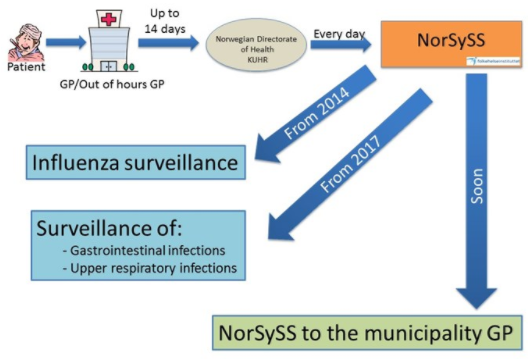
\includegraphics[width=16cm]{NorSySS_diagram}
\centering
\caption{NorSyss's process}
\label{fig:norsyss}
\end{figure}

The main suggestion of this thesis is as influenza develops it reveals subtle patterns in societal behaviors that is detectable through a variety of mediums, e.g urban datasets from sewage, public transportation, medicinal purchases, recreational habits, social media and other such sources of public information. With this suggestion, a tool to collect urban spatial datasets is needed and to present and visualize this information to best divulge the effect of the viral composition. The datasets used in this thesis is explained more in chapter 3, they consist however of the NIPH ILI and virus observations, the different datasets from the NPRA showing traffic patterns, social media of Twitter reporting symptoms directly from the public of Norway and two public transportation providers of the cities Stavanger and Oslo. Unfortunately more datasets could not be obtained within the time-scope of this thesis, but nonetheless, they provide a solid basis for examination and development.

\section{Outline}
The thesis is structured into seven chapters.
\newline \\Chapter 2 describes related works of what others have found useful as tools and other proven effective measurements.
\newline \\Chapter 3 marks out in detail the datasets used by this project, describes and give an explanation of relevance, challenges, limitation, and rewards.
\newline \\Chapter 4 outlines the implementation and graphical results of the datasets used in chapter 3.
\newline \\Chapter 5 shows the overall results.
\newline \\Chapter 6 discusses the results.
\newline \\Chapter 7 concludes the thesis, discusses constraints and possible future work as well as other suggestions.

\chapter{Related Works}
\section*{2.1 TODO}

\chapter{Experimental}
In this chapter, the different datasets used will be introduced. The goal of this thesis is to use as many datasets possible and then later evaluate them according to relevant results.

\section{The Norwegian Institute of Public Health}
The Norwegian Institute of Public Health (NIPH) have weekly updates\cite{fhi} on the development of the current influenza season as well as previous ones. The reports include numbers of diagnoses from general practitioners (GPs) considering influenza-like illness (ILI), and hospitalized virus observations. These are the main focus and acts as a baseline for other datasets to compare against. The virus observation numbers are included in the report, ILI symptoms are not, they are however both included in graphs. Upon further request, the ILI data was provided for the season of 2016/2017, and for the cities of Oslo and Bergen of the season of 2015/2016, 2016/2017 and 2017/2018. Exact numbers of the virus observations are only included for the three last years, therefore this thesis only uses the seasons of the years 2015/2016, 2016/2017 and 2017/2018. The reports also cover what kind of influenza viruses are circulating in the country and where, vaccine status and recommendations, as well as the overall prognosis of the current season. GPs report ILI based on these characteristics: muscle pain, coughing, fever and the feeling of being sick. The ILI numbers are perhaps of more interest since they are more accessible than virus observations that only counts for hospitalization. These two datasets provide the measurement basis other datasets are held up against.

\section{The Norwegian Public Roads Administration}
The Norwegian Public Roads Administration (NPRA) have several different collections of data available for a number of different purposes \cite{vegvesenet}. The main motivation for traffical data in this thesis is the hypothesis that when people are ill they commute less and thus this shows when surveying statistical details. Freely on their website \cite{vegvesenet} there are a few interesting options. They have traffic information in the standard traffic management exchange data structure (DATEX), application programming interfaces (API), statistics in an extensible markup language (XML) and traffic index data relevant to the years before. It is important for this thesis that the data collected is on a weekly basis at least in order to compare it to the influenza data. It turned out that the data on their website did not suffice for this purpose, they only had a temporal resolution of months or years while this thesis needs a temporal resolution of weeks or better. The data given contained a set of traffic registration stations throughout Norway. Data provided was on a weekly basis and also on an hourly basis for a subset of the original traffic registration stations provided. With this statistics of the traffic amount and spatial bounds can be derived showing the possible correlation influenza can have on commuting traffic. The regions of interest are the whole of Norway and the three cities of Stavanger, Bergen, and Oslo.

\section{Twitter}
The reason twitter data is interesting is that it contains self-reported instances of influenza on an individual level. These self-reported cases may even occur without the patient visiting a doctor, and so capture otherwise non-reported instances of ILI. The advantages are an instant notification about possible ILI and its spread, against the disadvantages of it being self-reported and thus somewhat unreliable. Twitter has several APIs available for public use, the one used in this project is the representational state transfer (REST) API or 'search API' which allows for searching against a set of keywords. The REST API is limited though, data accessible is roughly only maximum 10 days old and the search limit is on a maximum of one hundred messages called 'tweets'. The other API of interest is the stream API which continually gets the latest tweets. In order to only get Norwegian tweets, a set of geographical locations needs to be defined. The reason the stream API was not used is firstly that it requires a computer running on the internet continuously in order to get all the desired tweets. Secondly, the data collected could become large slowing down other post-processing algorithms and taking up unnecessary storage. Lastly, the stream API only provides a small set of the actual tweets tweeted, this means when searching for a specific term using the stream API some relevant tweets could go unnoticed and thus a search API is more appropriate for this task.

\section{Kolumbus}
Kolumbus is the public transportation administration in the state of Rogaland in Norway, this includes Stavanger, a city of interest. Unfortunately, Kolumbus provides no API, but on further request data of monthly passenger travel was provided from the years of 2015-2017.

\section{Ruter}
Ruter is the public transportation administration in the state of Oslo in Norway. Unfortunately, Ruter's API does not include passenger or tickets sold information, this was however provided on request for the years 2015, 2016, 2017 and up till 27 of February for the year 2018 on a daily basis.

\chapter{Implementation}
This chapter describes how the use of the different datasets were implemented and presented. The program is divided into two: The backend and the frontend. The structure and functions are provided by the backend, which governs collection and manipulation of data, and the frontend presents the data in a graphical user interface (GUI) using graphs and maps. Figure \ref{fig:program} show the structure and relations of the backend and the frontend in a simplified manner. The main module to be run is found in frontend/gui.py, and the system works best with two API keys installed as explained in this chapter.

\begin{figure}[h]
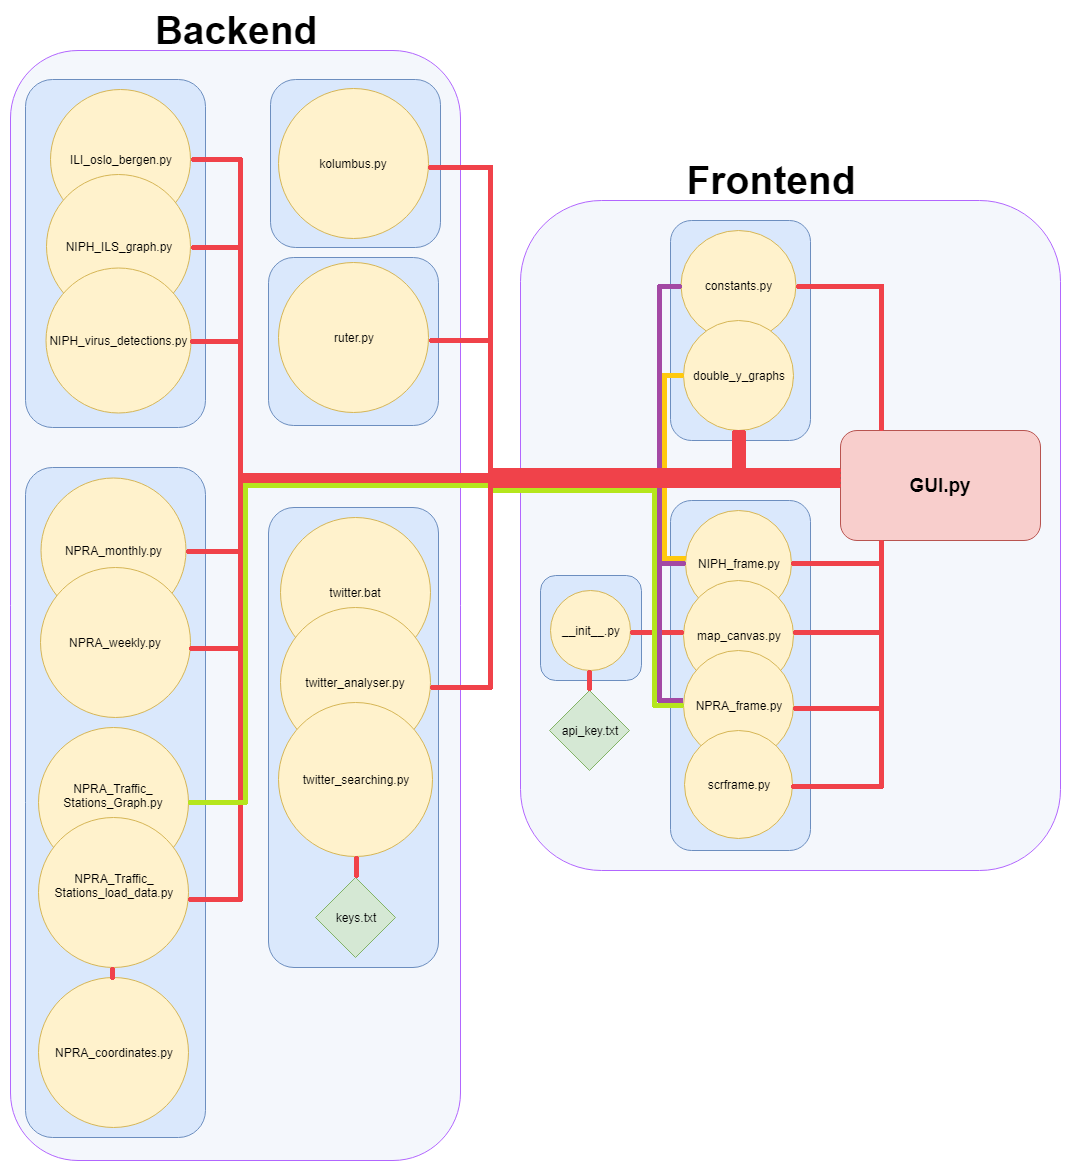
\includegraphics[width=11cm]{program_diagram}
\centering
\caption{Simplification of the overall program structure and relation}
\label{fig:program}
\end{figure}

\section{The Backend}
The backend is responsible for providing the frontend all the data and deeper functions it needs to visualize and administrate data to be show in graphs. The backend is partitioned into modules (Python programs/.py files) in their respective directory folder based on each dataset available. Each module may also be run individually for testing and easy viewing purposes. 
The Twitter module is unique as it requires 4 application programming interface (API) keys to work properly. The instructions for this set-up is found in the file README.md in the twitter module's directory.




\subsection{The Norwegian Institute of Public Health}
There are three different sets of data, which is divided into the separate modules of NIPH\_ILS\_graph.py, NIPH\_virus\_detections.py and ILI\_oslo\_bergen.py located in the same directory backend/NIPH, and they show influenza-like illnesses (ILI), hospitalized viral observations and more detailed ILI from the cities of Oslo and Bergen. The ILS module extract data from a local file, the virus module has it's data hard-coded and the ILI module extracts it's data from a hidden file (more on this in chapter 6), and they all draw their graph(s) using Python's matplotlib library. The graphs can be seen by running the modules individually or in the frontend main program frontend/gui.py's appropriate viewport accessible from the NIPH button. Figure \ref{fig:infstat} show the three last seasons of influenza in regards to observed viral infections. The plotting was done manually as NIPH only provides viral observational data in reports that are in pdf files on their official website\cite{fhi}.

\begin{figure}[h]
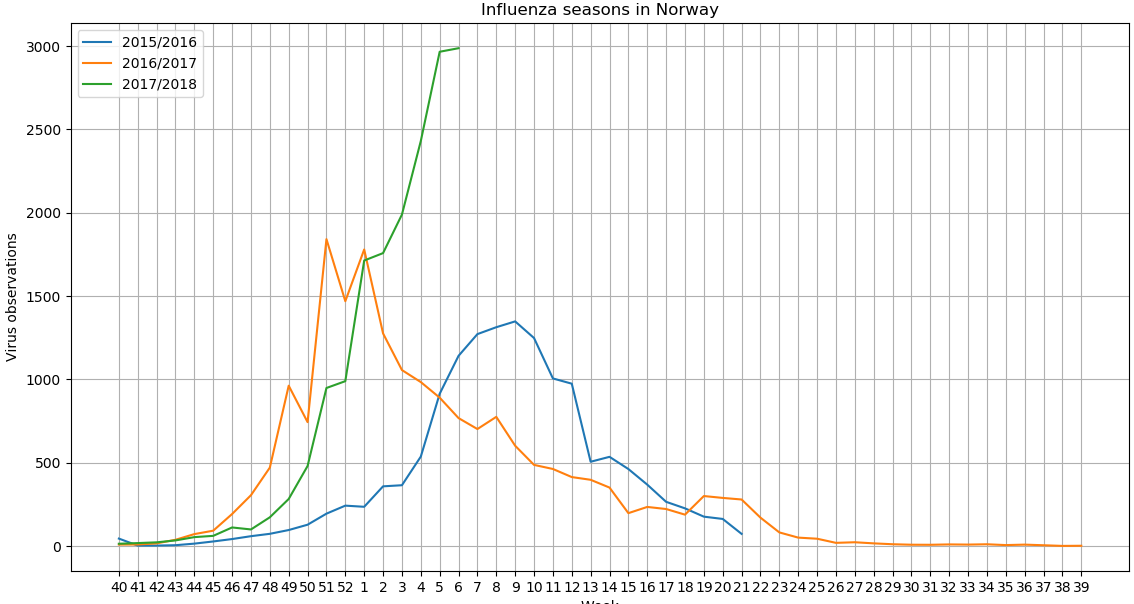
\includegraphics[width=12cm]{influenza_15_till_18}
\centering
\caption{Influenza virus observation}
\label{fig:infstat}
\end{figure}

Figure \ref{fig:ilsstat} shows the influenza-like illnesses (ILI) of the year 2016/2017. This was not done manually as data was provided in a simple .xlsx file which was read using Python's openpyxl module, processed and then drawn as a graph. Figure \ref{fig:ili_oslo} and figure \ref{fig:ili_bergen} show reported ILI from Oslo and Bergen.

\begin{figure}[ht]
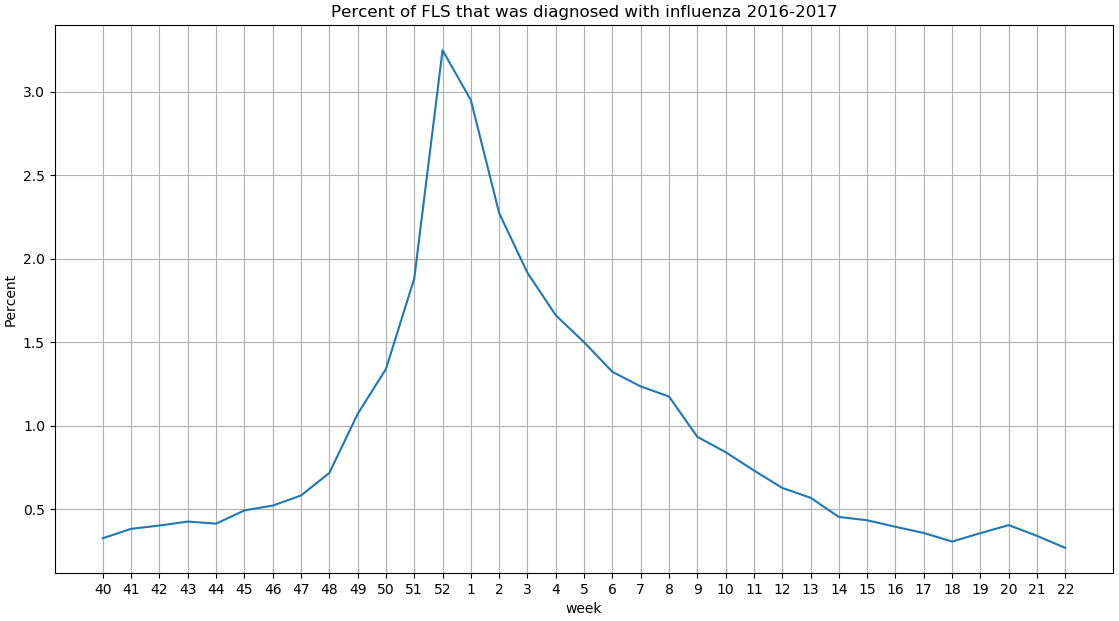
\includegraphics[width=12cm]{ILS_16_till_17}
\centering
\caption{Influenza-like illnesses season 2016/2017}
\label{fig:ilsstat}
\end{figure}

\begin{figure}[ht]
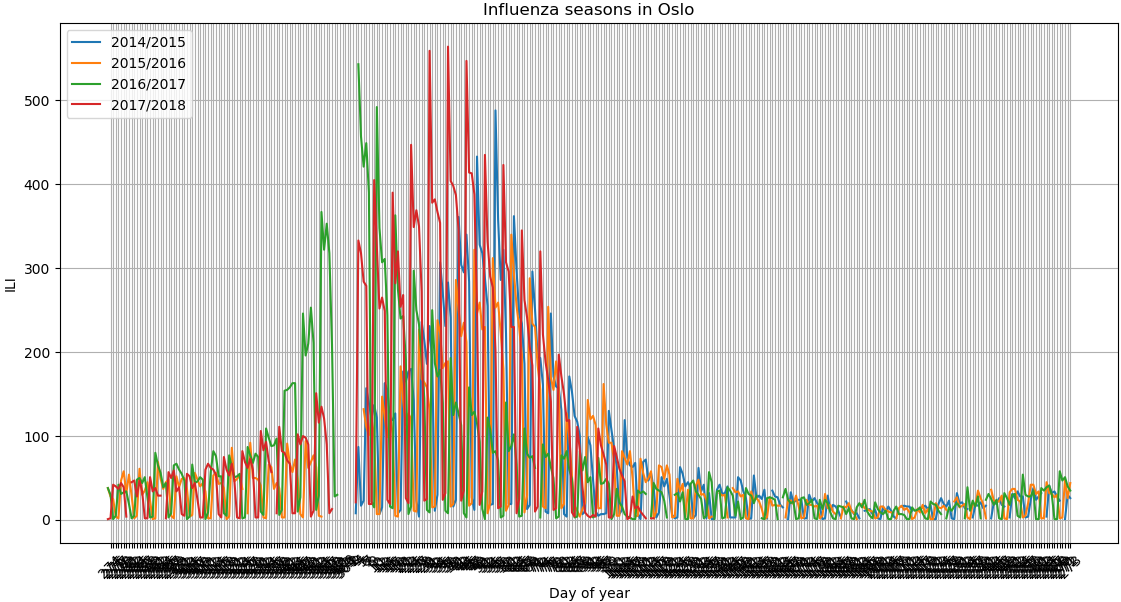
\includegraphics[width=12cm]{ili_daily_oslo}
\centering
\caption{Influenza-like illnesses season 2014-2018 in Oslo}
\label{fig:ili_oslo}
\end{figure}

\begin{figure}[!htb]
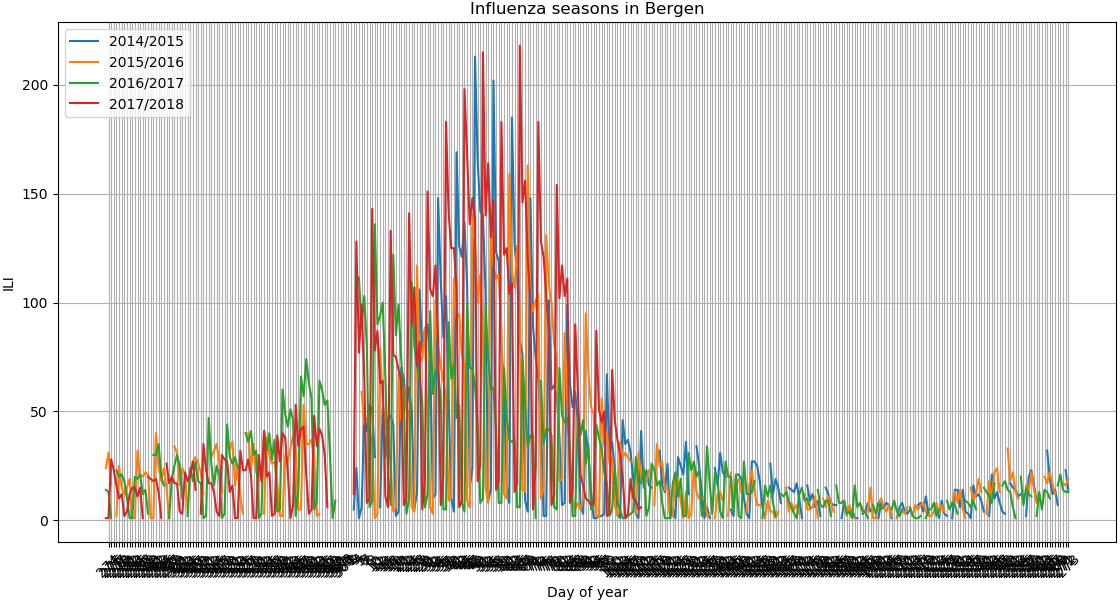
\includegraphics[width=12cm]{ili_daily_bergen}
\centering
\caption{Influenza-like illnesses season 2014-2018 in Bergen}
\label{fig:ili_bergen}
\end{figure}

\newpage









\subsection{The Norwegian Public Roads Administration}
From the .xlsx files provided by the NPRA, simple graphs were created in python showing the total annual traffic on Norwegian roads from 2002 to 2015 on a monthly basis as seen in figure \ref{fig:anualtotal}.

\begin{figure}[ht]
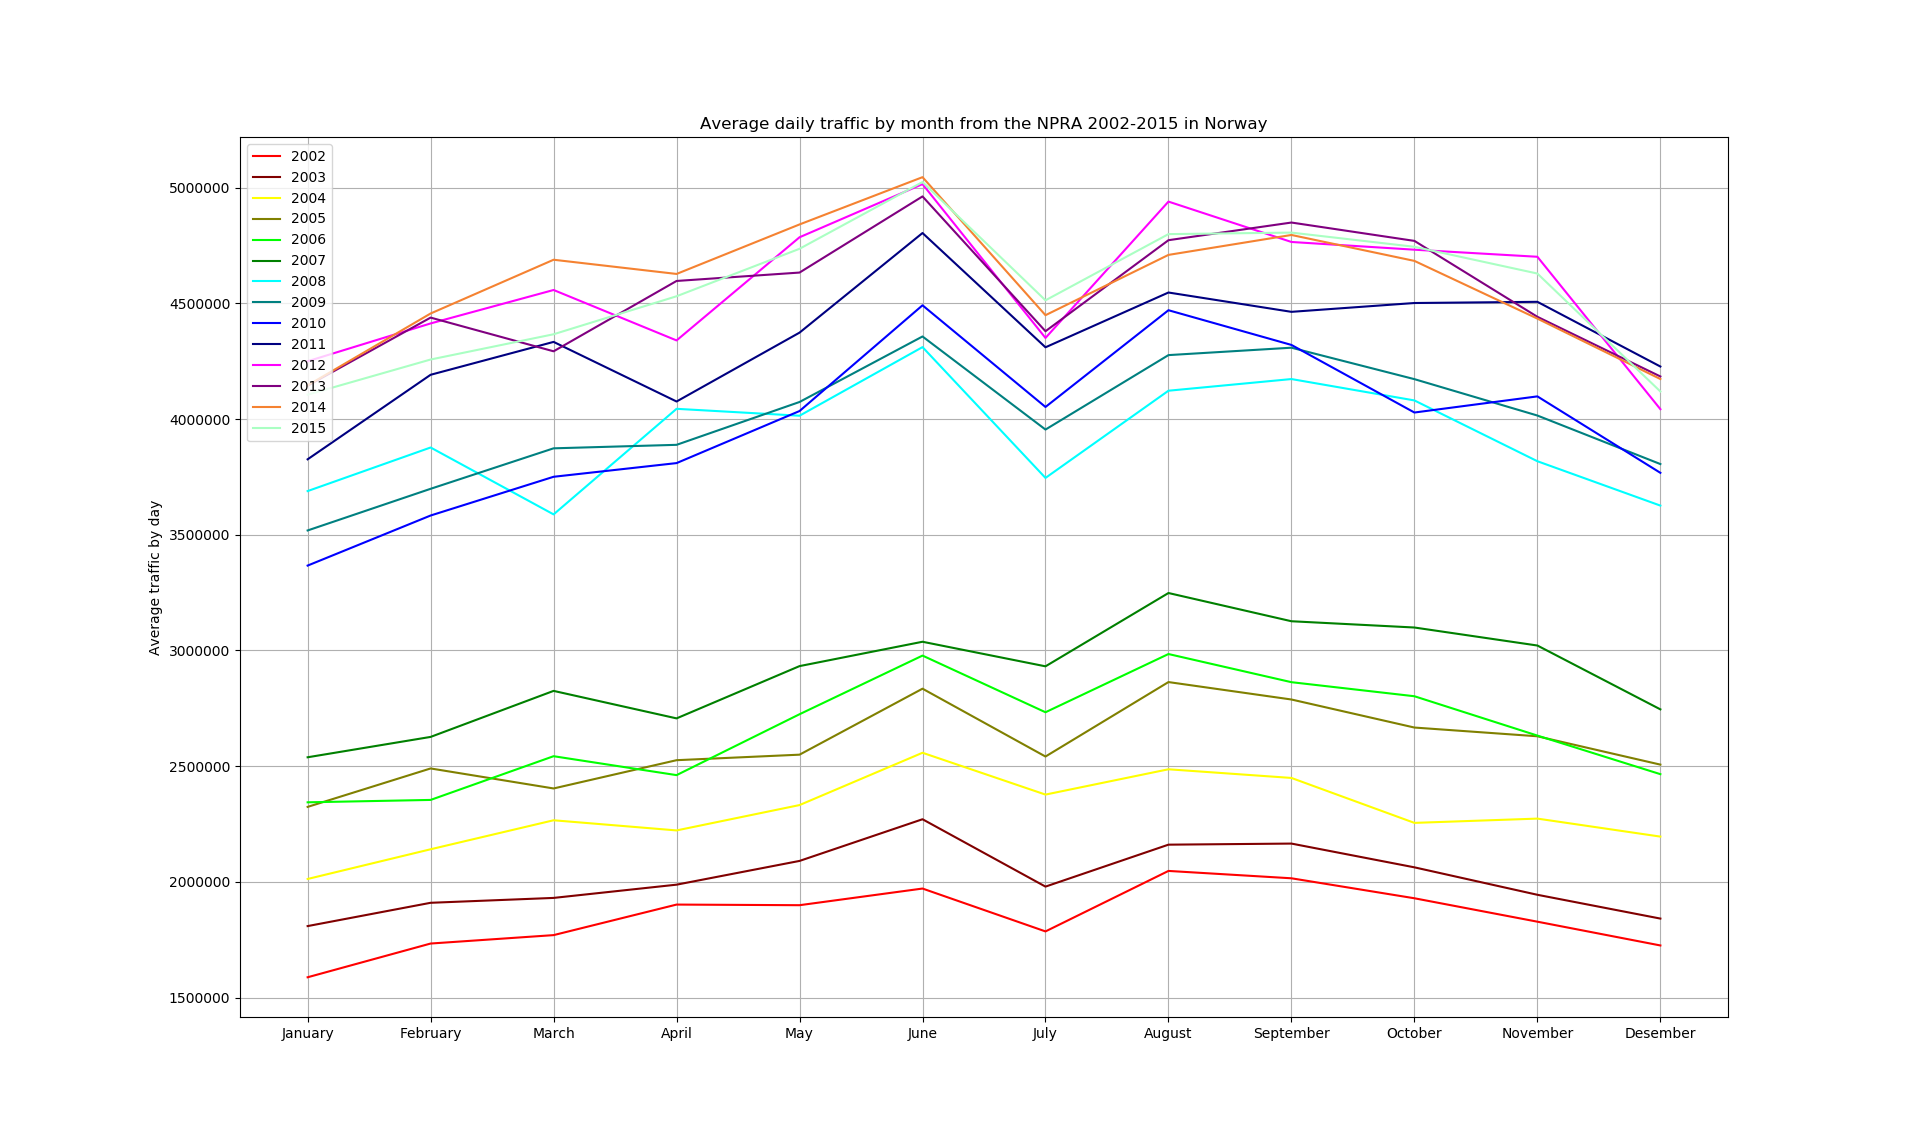
\includegraphics[width=12cm]{xml_02_15_annual_total}
\centering
\caption{Annual traffic 2002-2015}
\label{fig:anualtotal}
\end{figure}

Also derived from this dataset is the annual traffic of the two cities of Bergen and Oslo, which are cities of interest.
%Figure \ref{fig:anualbergen} shows the traffic in Bergen, and figure \ref{fig:anualoslo} show the traffic in Oslo.

%\begin{figure}[ht]
%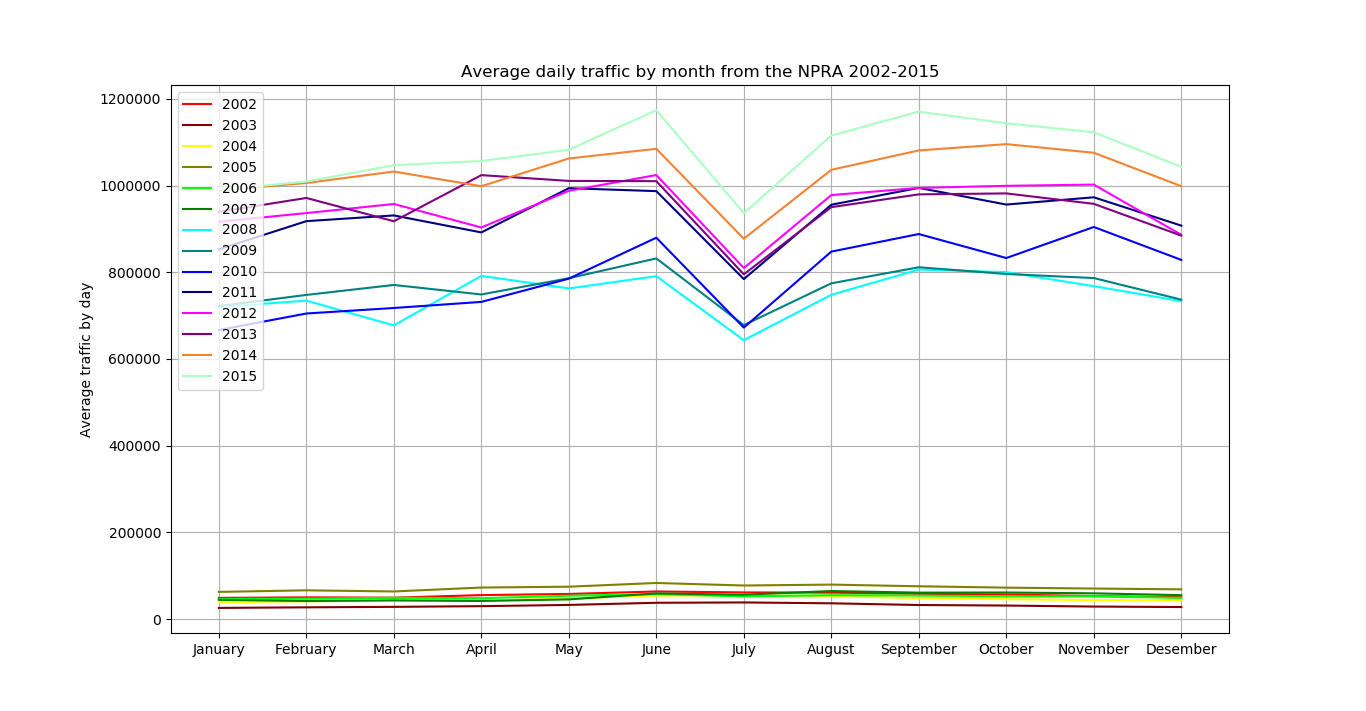
\includegraphics[width=12cm]{xml_02_15_annual_bergen}
%\centering
%\caption{Bergen traffic 2002-2015}
%\label{fig:anualbergen}
%\end{figure}

%\begin{figure}[ht]
%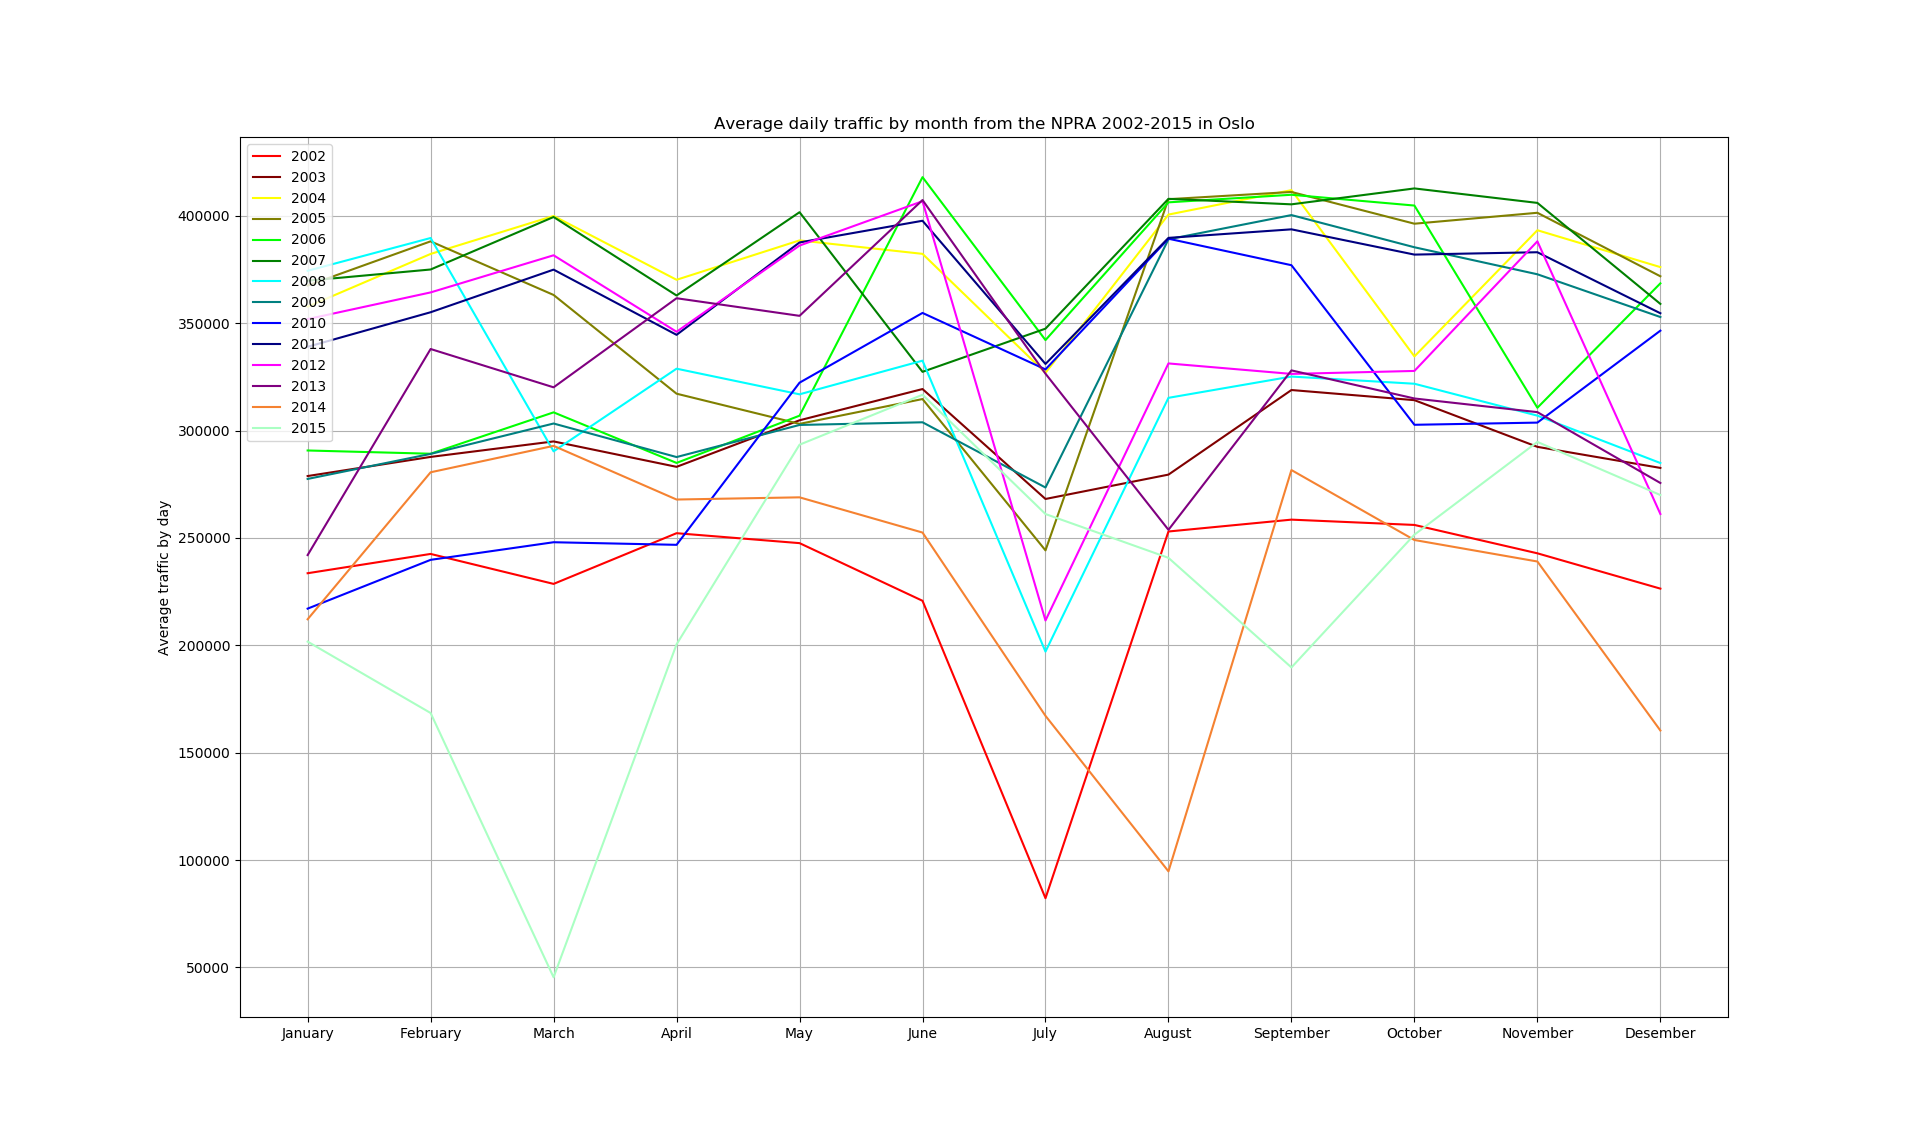
\includegraphics[width=12cm]{xml_02_15_annual_oslo}
%\centering
%\caption{Oslo traffic 2002-2015}
%\label{fig:anualoslo}
%\end{figure}
The dataset is in an XML file structure, a module named NPRA\_monthly.py was created that reads through all rows and collects the relevant columns into an array using Python's openpyxl module and then draws a graph using Python's matplotlib module. For the annual graph, every month of every year was collected. For the towns of Bergen and Oslo the correct roads were identified and then every year of every month of those roads was collected, loaded into an array and then drawn as a graph. The separate text files 'Bergen places.txt' and 'Oslo places.txt' is to make it easy to edit should these roads change in the future. This module when run individually accepts one command argument from the user, either cities of Oslo or Bergen may be provided to specify interest, if no argument is given the annual graph will show. The problem of using these datasets is that the data is an average calculation of monthly traffic, meaning the temporal bounds are too coarse for comparison against the influenza data which in turn is on a weekly basis. For these reasons no figures of this dataset are shown in this thesis (except figure \ref{fig:anualtotal}), they are however available as modules in the directory backend/NPRA/NPRA\_monthly.py and can be seen in the frontend's main program frontend/gui.py appropriate viewport accessible from the NPRA button.

For the weekly datasets a set of traffic registration stations was needed to define the temporal bounds of each area of interest. Defined are the towns of Oslo, Stavanger, and Bergen, as well as the whole of Norway on a level 1 basis. The level 1 registrations are continuous throughout the year on an hourly basis and is exactly what this thesis requires. The module NPRA\_weekly.py captures these functions and also provides the user with command arguments if run individually. The commands are the cities of Bergen, Stavanger or Oslo, if no commands are given the annual graph of the whole of Norway will be drawn instead.

Figures \ref{fig:weeklybergen}, \ref{fig:weeklyoslo} and \ref{fig:weeklystavanger} shows the traffic on a weekly basis. This provides a better resolution for better analysis.
\begin{figure}[ht]
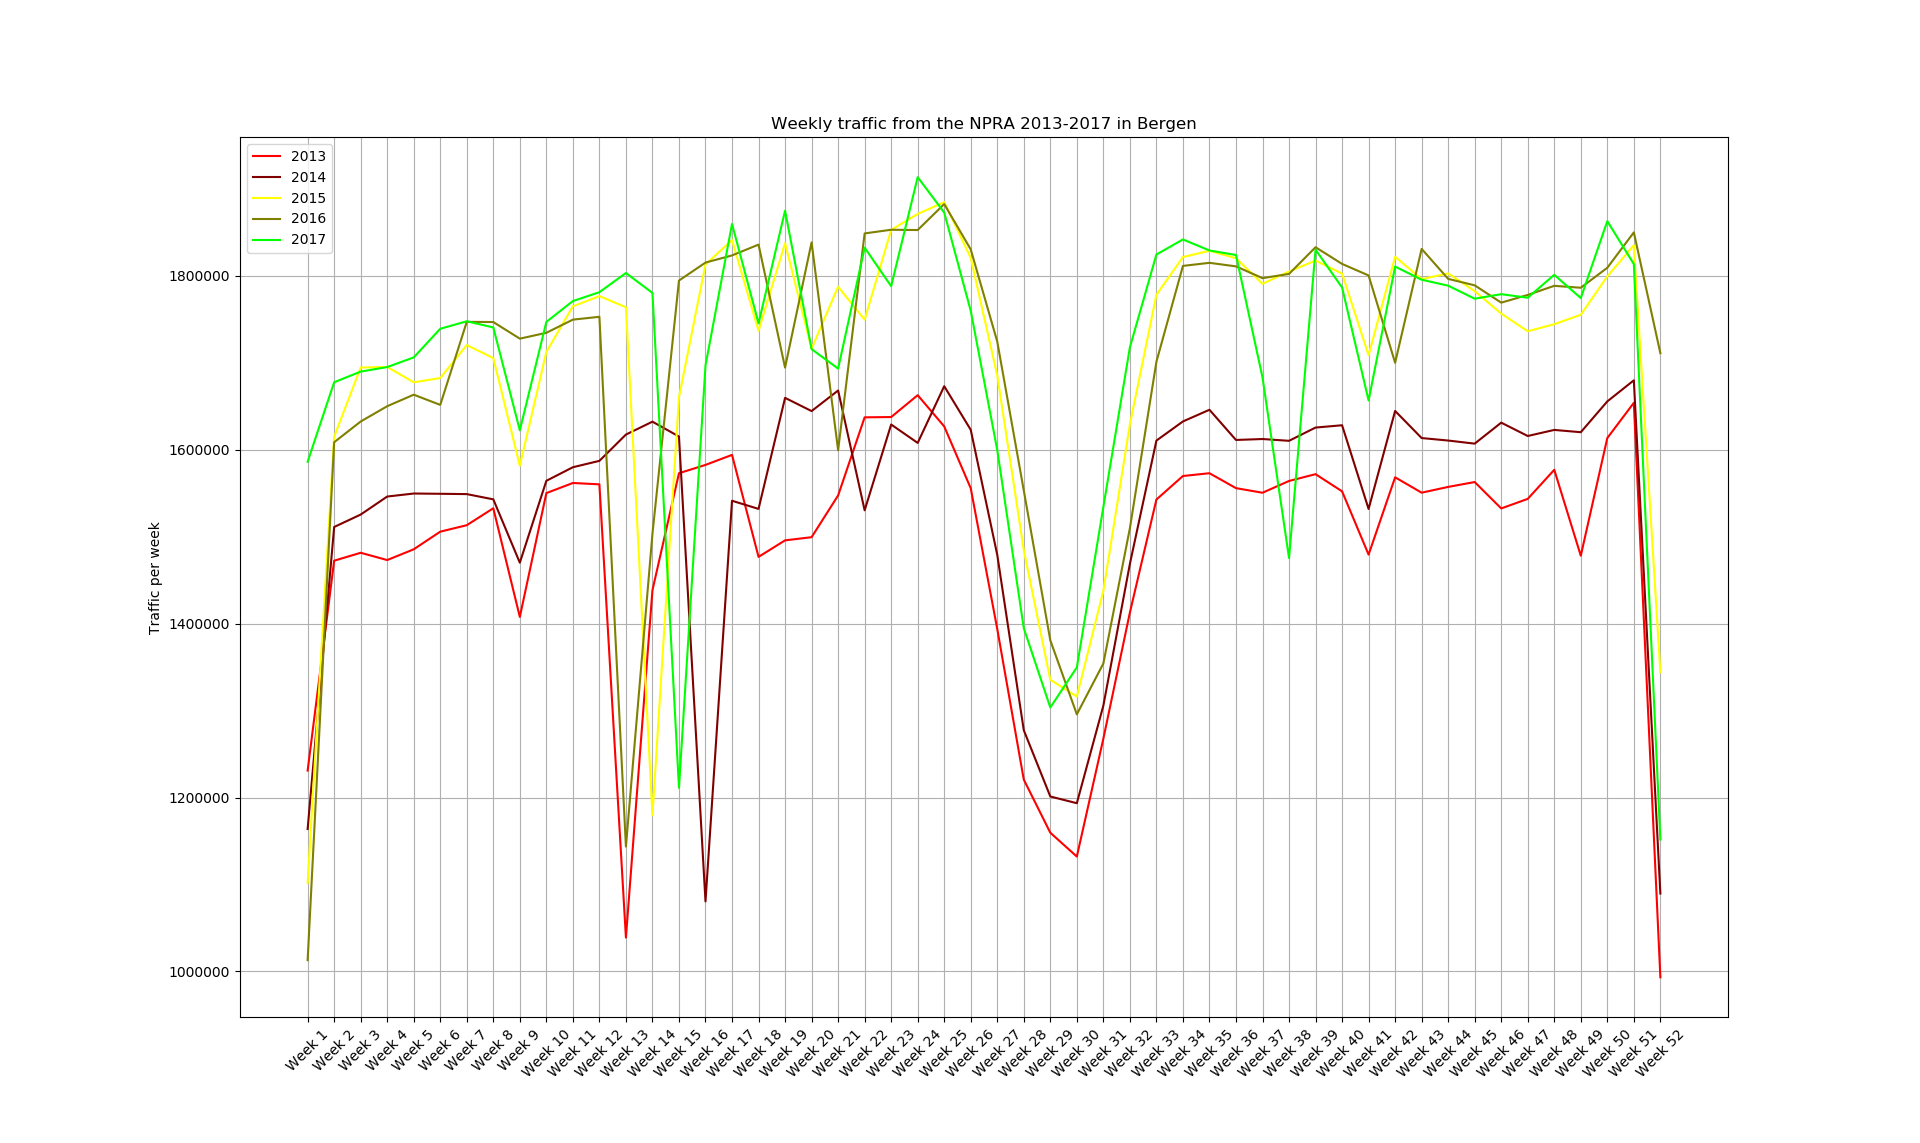
\includegraphics[width=12cm]{NPRA_13_17_weekly_bergen}
\centering
\caption{Weekly data of the city of Bergen}
\label{fig:weeklybergen}
\end{figure}

\begin{figure}[ht]
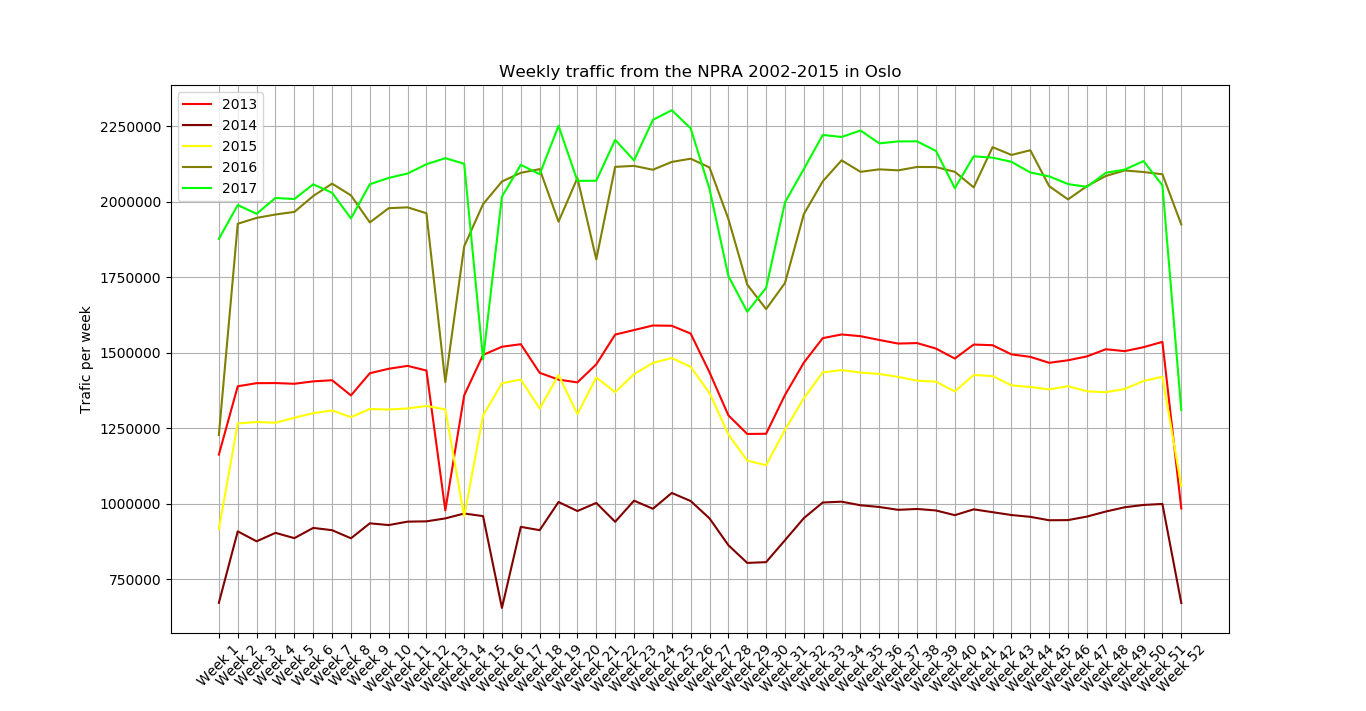
\includegraphics[width=12cm]{NPRA_13_17_weekly_oslo}
\centering
\caption{Weekly data of the city of Oslo}
\label{fig:weeklyoslo}
\end{figure}

\begin{figure}[ht]
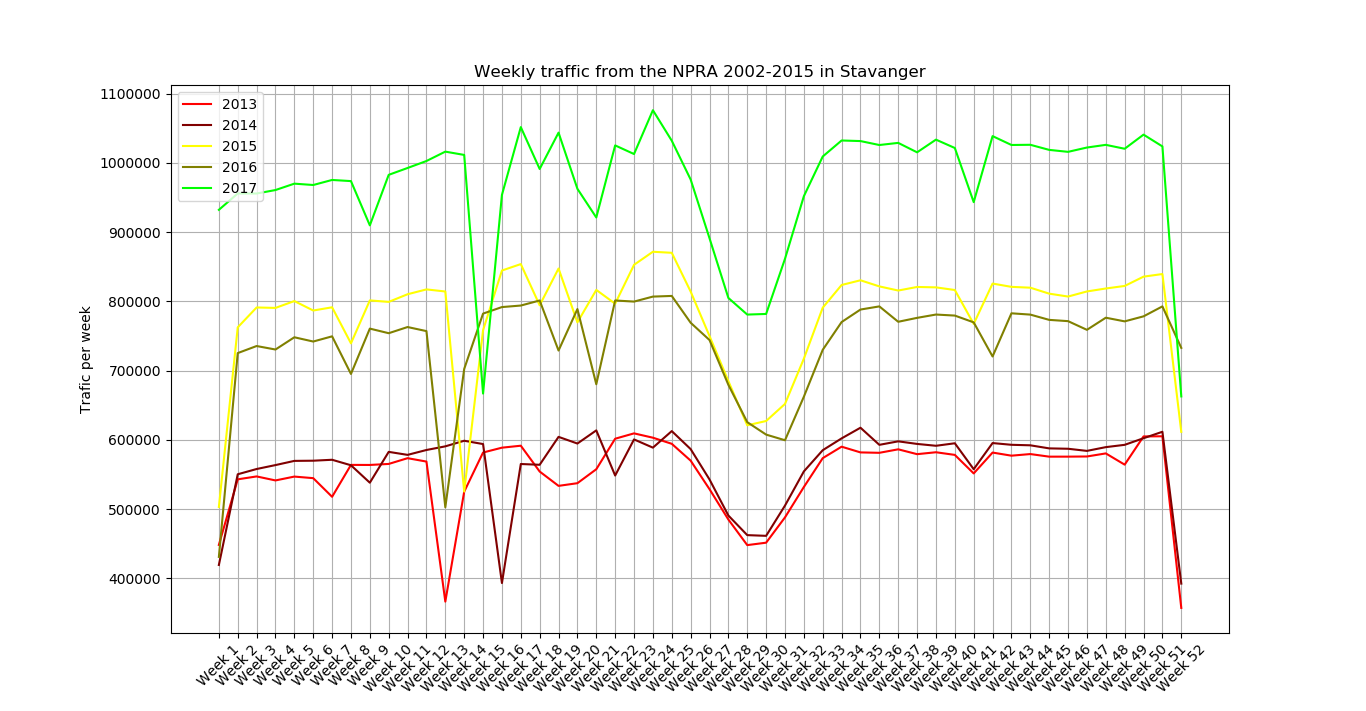
\includegraphics[width=12cm]{NPRA_13_17_weekly_stavanger}
\centering
\caption{Weekly data of the city of Stavanger}
\label{fig:weeklystavanger}
\end{figure}

Figure \ref{fig:boundsbergen}, \ref{fig:boundsoslo} and \ref{fig:boundsstavanger} shows the different geospatial bounds used to define the cities, and the respective data from traffic registration stations was collected from these. The green circles with numbers inside show where and how many traffic registration stations there are.

\begin{figure}[!htb]
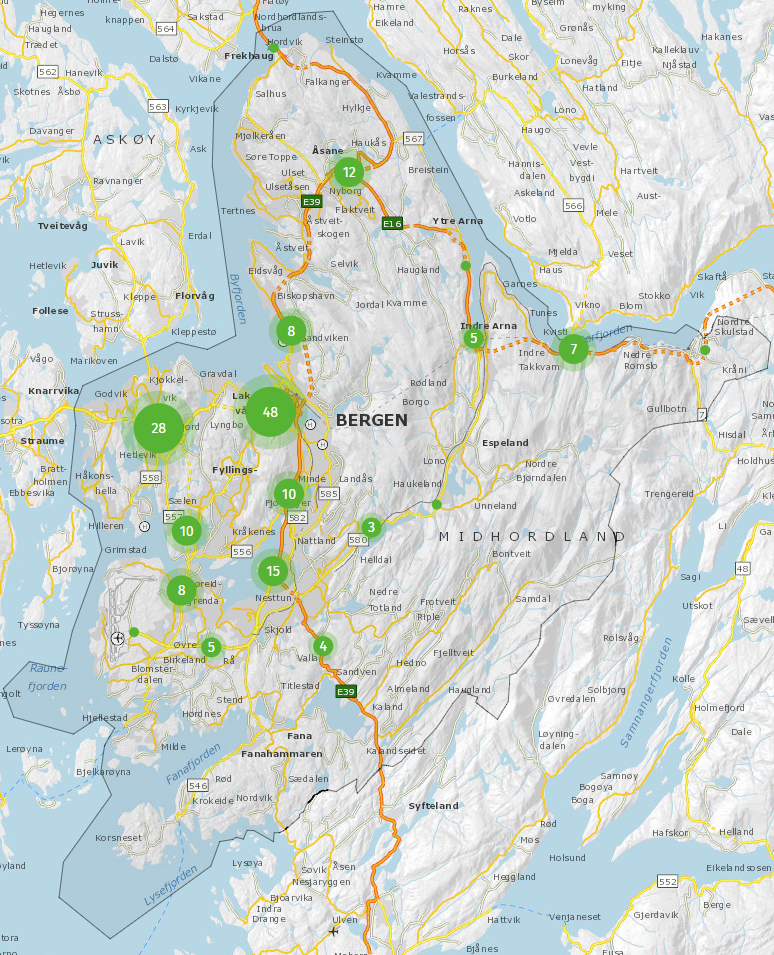
\includegraphics[width=10cm]{nivaa_1_bergen}
\centering
\caption{Geospatial bounds of Bergen, used for weekly data. The green circles show where the traffic registration stations are, and the number reveals how many there are in that general area.}
\label{fig:boundsbergen}
\end{figure}

\begin{figure}[!htb]
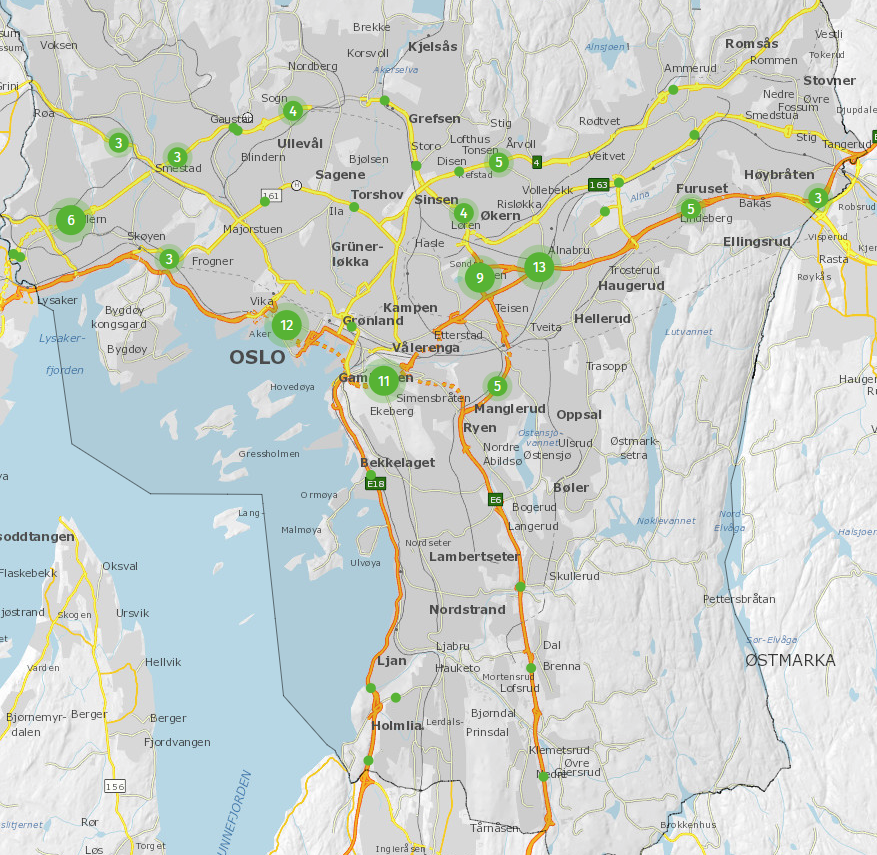
\includegraphics[width=10cm]{nivaa_1_oslo}
\centering
\caption{Geospatial bounds of Oslo, used for weekly data. The green circles show where the traffic registration stations are, and the number reveals how many there are in that general area.}
\label{fig:boundsoslo}
\end{figure}

\begin{figure}[!htb]
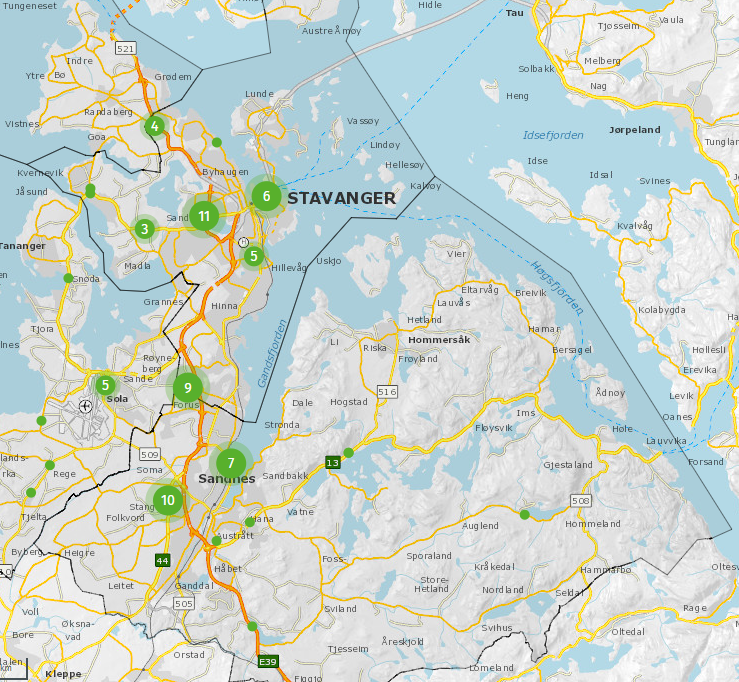
\includegraphics[width=10cm]{nivaa_1_stavanger}
\centering
\caption{Geospatial bounds of Stavanger, used for weekly data. The green circles show where the traffic registration stations are, and the number reveals how many there are in that general area.}
\label{fig:boundsstavanger}
\end{figure}

The last NPRA dataset acquired was raw hourly data from a defined subset of all of NPRA's traffic registration stations previously used, this is because the NPRA would only provide this much data from their stores. The data contains all whole hours from all weeks over several years, number of fields available on the road (vehicle lanes, usually only two for regular roads), and how many vehicles passed by that hour and also their lengths in category. Figure \ref{fig:hboundsbergen}, \ref{fig:hboundsoslo} and \ref{fig:hboundsstavanger} shows the different geospatial hourly based bounds (traffic registration stations) used. There are two modules dedicated to the hourly datasets, the NPRA\_Traffic\_Stations\_Graph.py and the NPRA\_Traffic\_Stations\_load\_data.py found in the directory
Backend/NPRA/Traffic\_registration\_stations/hourly\_datasets. The graph module is responsible for drawing a graph with specifications of hour to/from, weekday to/from, month to/from, year and field. The load data module is responsible for providing the graph with all the functions it needs to operate, like querying the dataset, the variance of the queried dataset, extracting the dataset from file and organizing it into a data structure, and reading and handling the coordinates of the traffic registration stations so that it can be shown on the map. These last hourly based datasets provide high quality information and is presented in the GUI, by clicking the NPRA button, where the user can try different queries to find different information, more explanations follow in the frontend section of this chapter.

\begin{figure}[!htb]
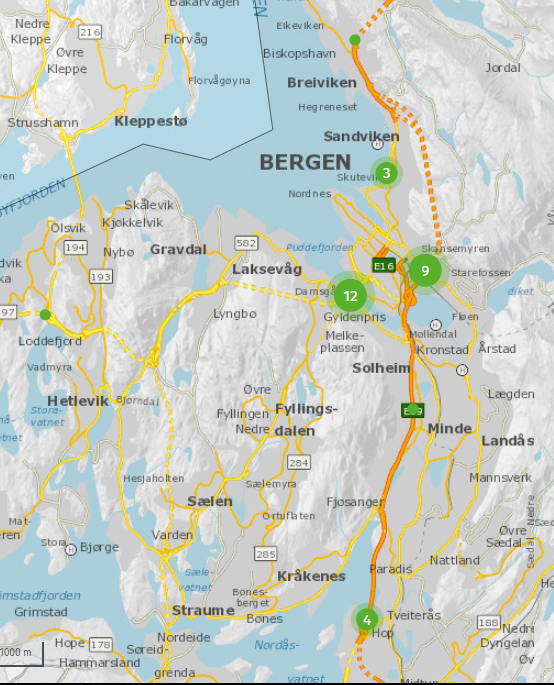
\includegraphics[width=10cm]{times_nivaa1_BERGEN}
\centering
\caption{Geospatial hourly bounds of Bergen, used for hourly data}
\label{fig:hboundsbergen}
\end{figure}

\begin{figure}[!htb]
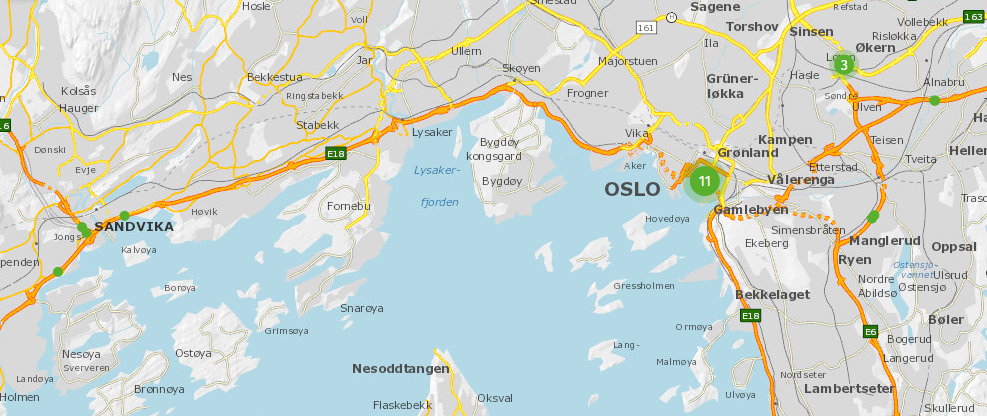
\includegraphics[width=10cm]{times_nivaa1_OSLO}
\centering
\caption{Geospatial hourly bounds of Oslo, used for hourly data}
\label{fig:hboundsoslo}
\end{figure}

\begin{figure}[!htb]
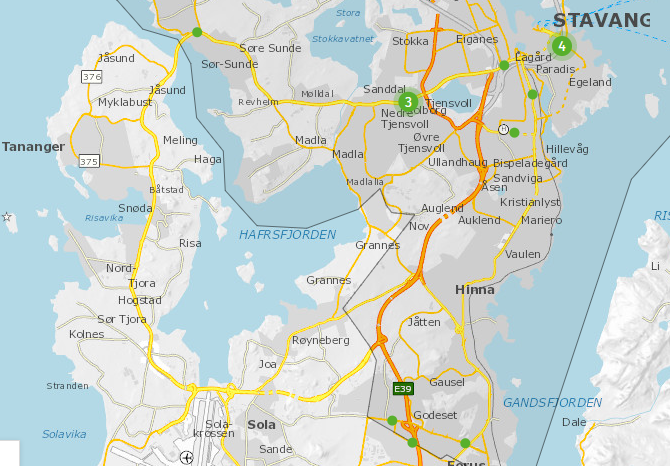
\includegraphics[width=10cm]{times_nivaa1_STAVANGER}
\centering
\caption{Geospatial hourly bounds of Stavanger, used for hourly data}
\label{fig:hboundsstavanger}
\end{figure}

\newpage







\subsection{Twitter}
Using the representational state transfer (REST) application programming interface (API) it was paramount that in order to build a sufficient dataset, acquiring and collecting data had to begin as soon as possible in order to collect enough data for this thesis. A simple python module was created that takes the input of the API keys provided by the file keys.txt and the keywords to be searched upon provided by the file search\_terms.txt. Explanation on how to create the API key is found in the file backend/twitter/README.md. The program ensures that some duplicate messages are ignored but not all (explained more in the following chapter), and the limit of a hundred tweets dictated by the REST API user agreement was overcome simply by searching for yet another hundred from the last date of the previous hundred until the date limit of about 10 days was reached.
The output is appended to a file in this data structure on new lines: id, date, location, tweet, there is also a dotted separator for each new tweet making it more easy for humans to read. The functions described are implemented by the file twitter\_searching.py, which can be run as its own module and saves new tweets to the file twitter\_data.txt.

A straightforward analysis tool for the Twitter data in the file twitter\_data.txt was created by simply counting how many tweets there are. The idea is that during influenza seasons numbers of influenza-related tweets increases and then decrease when off the season, while the number of non-relevant tweets is constant during the whole year (or slightly increasing or decreasing based on the popularity of Twitter as a social media). A more complex tool for analysing the tweets for relevance was elected to bee too much work for this thesis. The advantage of simply counting how many possible tweets there are is that it is fast and easy to implement, the drawback is that it captures non-relevant tweets. Future work may be done to improve this quality with a better analysis tool. Figure \ref{fig:twitterAnal} shows the results of the time-frame captured. The analysing function is implemented in the file twitter\_analyser.py, when the module is executed on its own it shows a graph over the data found in the file twitter\_data.txt. A simple batch file twitter.bat was created to make it easy running these programs in the desired order. This module requires manual updates by running the individual module itself in the directory backend/twitter/twitter.bat. If no API key is provided the Twitter graph can still be viewed in the frontend main program frontend/gui.py's appropriate viewport accessible from the Twitter button, but it cannot append new updates without this key.

\begin{figure}[ht]
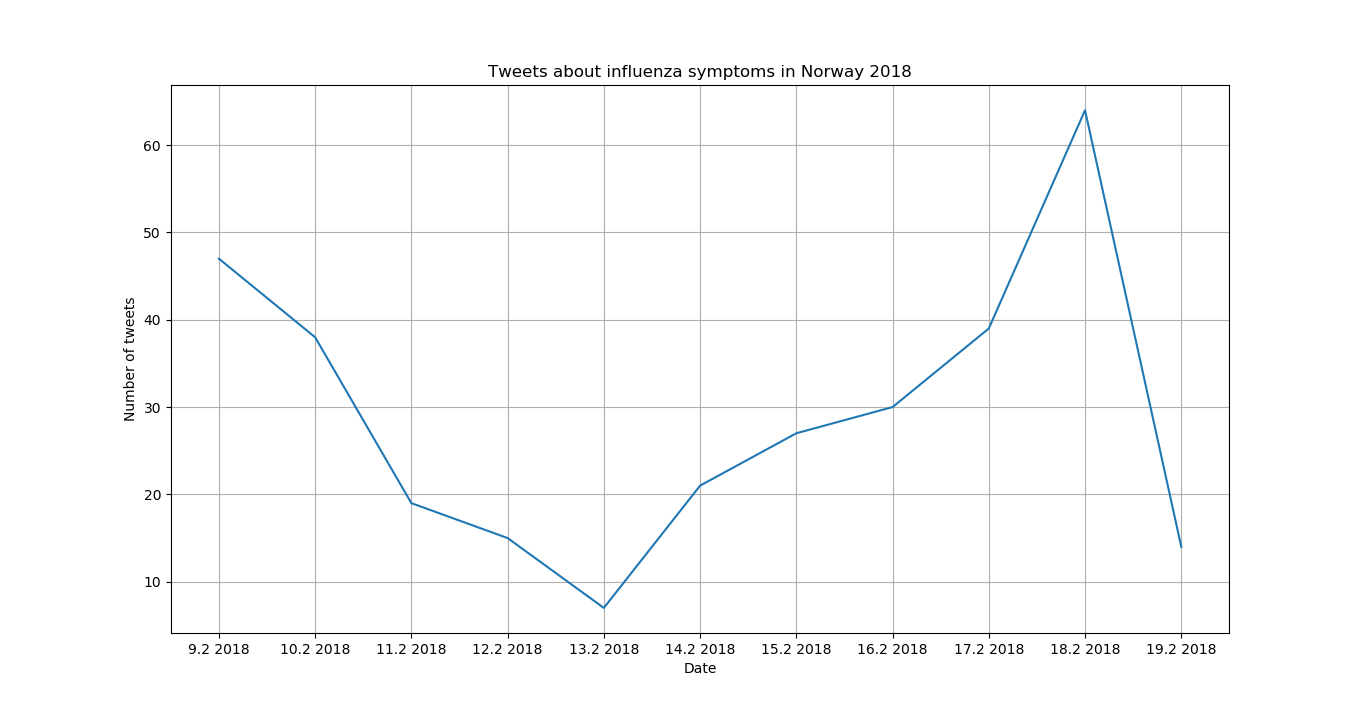
\includegraphics[width=16cm]{twitter_tweets_2018}
\centering
\caption{Tweets concerning ILS of 2018}
\label{fig:twitterAnal}
\end{figure}

\newpage







\subsection{Kolumbus}
The data provided by Kolumbus was in a .png format needed to be converted into a more convenient (and appropriate) data structure. The chosen data structure conversion was comma separated values (CSV) stored in the delimited text file '15\_17\_månedstall\_total.csv'. From there it was a simple job to plot the data in a python script, unfortunately the data is only on a monthly basis. Figure \ref{fig:kolumbus_15_17} shows the results.

\begin{figure}[!htb]
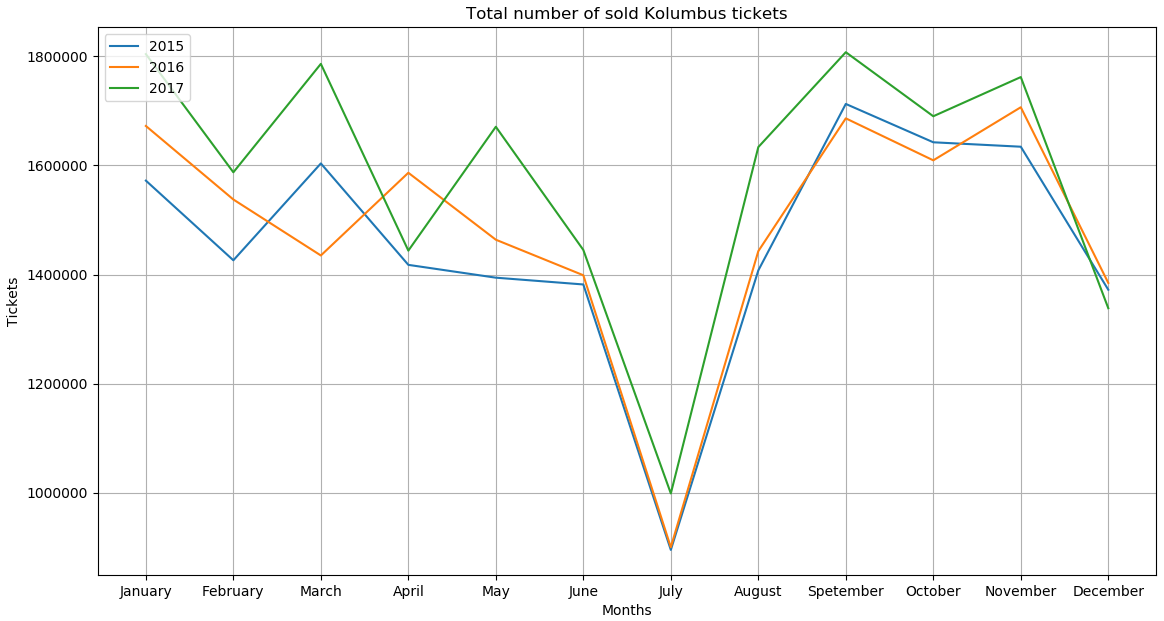
\includegraphics[width=11cm]{kolumbus_total_num_sold_15_17}
\centering
\caption{Monthly passenger travel with Kolumbus}
\label{fig:kolumbus_15_17}
\end{figure}







\subsection{Ruter}
The data provided by Ruter was in a .xlsx file and could easily be read, extracted and plotted by a simple python script. Figure \ref{fig:ruter_15_18} shows the results. Consider that with Python's matplotlib module, mounted in the frontend's main program frontend/gui.py, a user can zoom in and out to get a more desired and uncluttered view. The data was provided by a daily basis for the years of 2015-2018. Observe that the first year (in blue) is lower because it does not contain Oslo's underground train service passenger data.

\begin{figure}[!htb]
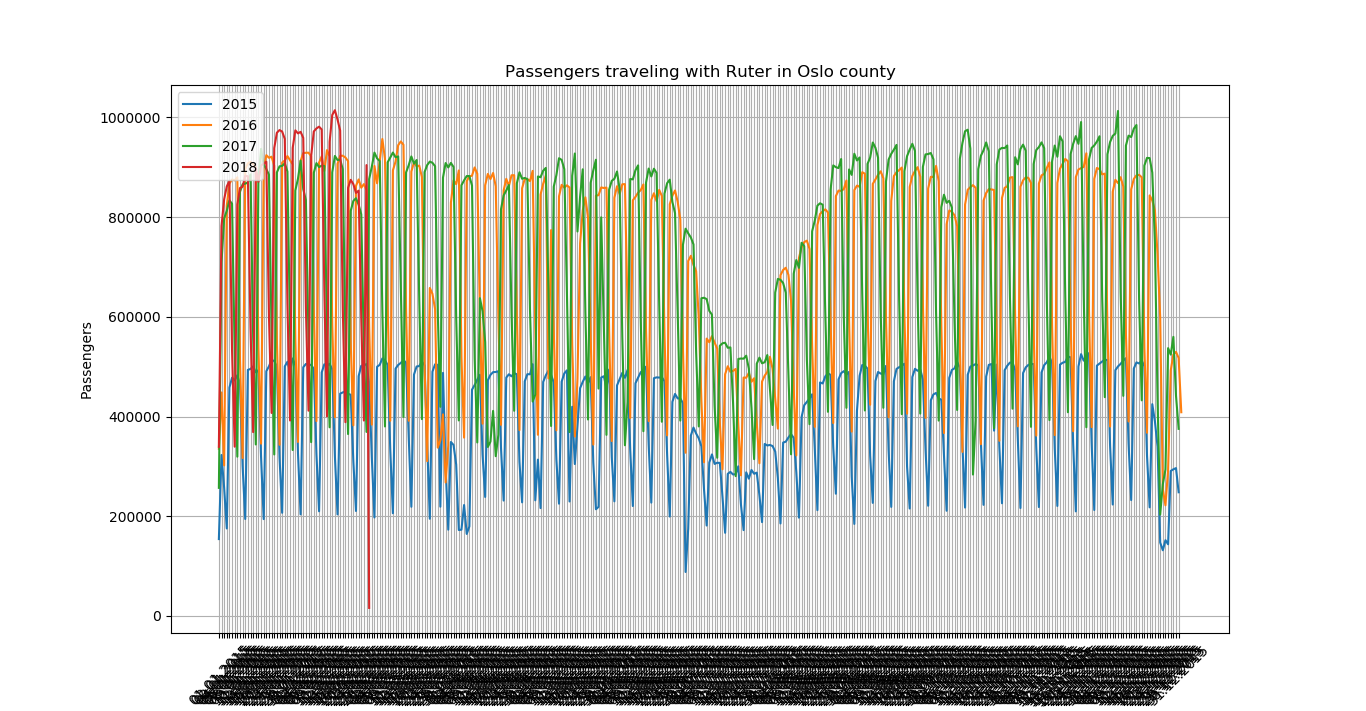
\includegraphics[width=11cm]{ruter_15_18}
\centering
\caption{Daily tickets sold with Ruter, the year of 2015 does not contain Oslo's underground train service passenger data}
\label{fig:ruter_15_18}
\end{figure}

\newpage










\section{The Frontend}
The thesis's program is divided into two: The backend and the frontend. The frontend is responsible for visualising the data provided by the backend. It does so by mounting a graphical user interface (GUI) that provides everything the user needs from this thesis. The GUI uses other frontend modules described in the following subchapters.

\subsection{The GUI}
The file gui.py is the main program. It mounts the GUI with help from backend modules and the frontend modules such as the file map\_canvas.py, the file scrframe.py, the file double\_y\_graphs.py, the file NIPH\_frame.py and the file NPRA\_frame.py . The GUI is created using Python's standard Tkinter module (standard meaning it's not a required external library), and it provides the means of a basic window creation with all the other usual GUI necessities available. 

The program gui.py is structured in two parts: The buttons frame and the data frame. The buttons frame produces a menu and simply makes available buttons to be clicked upon showing the different graphs for the respective datasets from the backend. The data frames show the graphs and if needed a map, visualizing the data from the backend. The backend takes time to load, to make this experience more user-friendly a progress bar is shown progressing relative to the actual loading sequence. Upon completion, the NIPH data is shown as a default view. The user may use the mouse wheel to scroll up and down the view and click the buttons to change datasets. 

In some datasets, a map is provided for further visualisation. the map is interactive with its own buttons and also responds to dragging the mouse in order to move the map, double-clicking in order to zoom in and using the mouse wheel, when hovering over the map, to zoom in and out. Figure \ref{fig:the_gui} shows the GUI.

\begin{figure}[!htb]
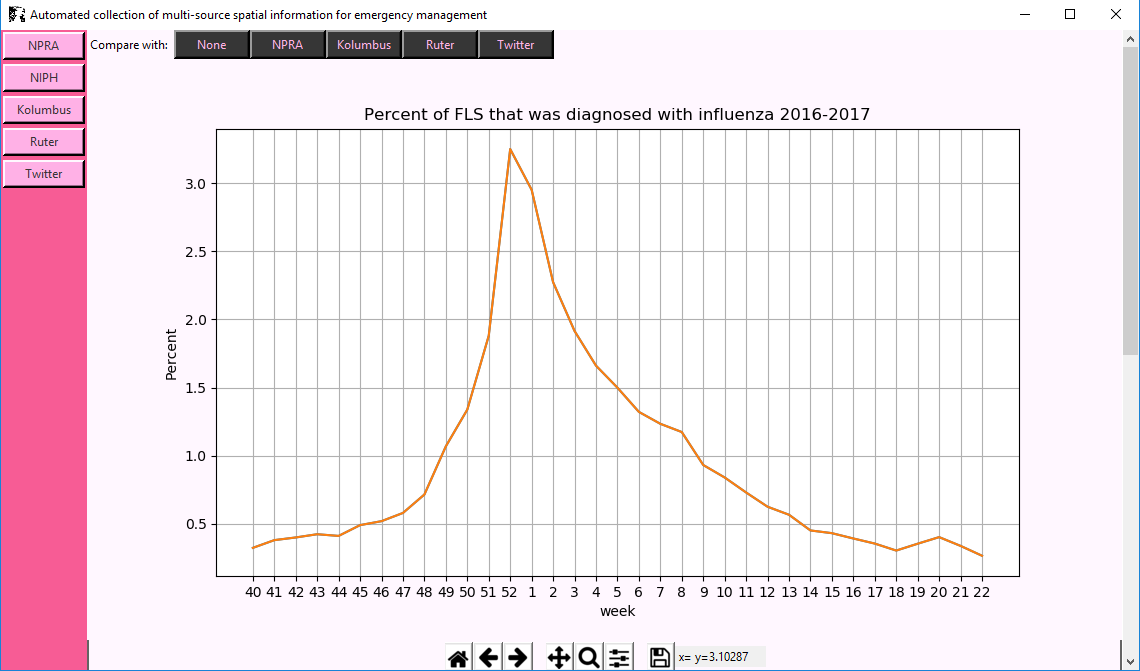
\includegraphics[width=12cm]{the_gui}
\centering
\caption{The GUI}
\label{fig:the_gui}
\end{figure}



\subsection{The Map}
The file map\_canvas.py provides the GUI a Goompy\cite{goompy} map on a Tkinter canvas. This file is also from the Goompy project, but is heavily modified to serve the purpose of this thesis. The file launches a Google static API map on a Tkinter canvas and provides basic Google map functions and user input. The functions edited for this thesis is: better zooming capabilities, coordination markers with individual colors and sizes, ability to focus on the map by will and some other minor bug fixes.

\subsubsection{Goompy}
Goompy\cite{goompy} is an open Github project and provides an interactive Google static map\cite{googleSM} for Python, it was created by Simon D. Levy. The main program uses this map implementation with it's own significant modifications to serve an interactive Google based map solution in order to provide visualisation of information.\\
The core Goompy file is found in the directory of /Frontend/goompy/\_\_init\_\_.py. This was heavily edited to provide the necessary functions of this thesis. The edit includes: Multithreading the fetching of Google static map images thus making Goompy about four times faster, dragging now changes latitude and longitude based on x and y position of the map to better help zooming functions, having the API key fetched from a separate text file in order to hide this from misuse by other developers, support of optional map coordinates to be plotted directly in the Google static map API, using and drawing a list of coordinates as a diamond-shaped polygon with individual colors and sizes and using the mouse wheel to zoom in and out.\\
The initial build fetched about one image per second in order to not exceed Google's throttle request quota. Upon further investigation this quota is set to ten QPS (queries per second) which means such a high buffer can be exploited. By converting the image extraction algorithm to be multi-threaded, fetching map fragments was increased to 4 - 6 images per second, well below Google's QPS and significantly strengthening the user experience by having a more responsive program.\\
Goompy requires a Google static map API key in order to work properly, users are asked to create the file Frontend/api\_keys.txt and paste the key there as described by the file Frontend/README.md. The original project saved the Google map images in a cache so that fetching a specific map with a familiar geolocations would be instantaneous instead of fetching them again from the Google server, this however was a violation of the terms of agreement and that function was removed from this thesis. Caching resources is a good way to quickly get often used functions, although the new implementation changes latitude and longitude often, as it allows this change, this is no longer a good strategy. For these two reasons the caching was removed.
Figure \ref{fig:the_goompy} shows the Goompy map interface. In the top left corner radiobuttons change the current viewing map type. The buttons to zoom in and out are found in the bottom right corner.

\begin{figure}[!htb]
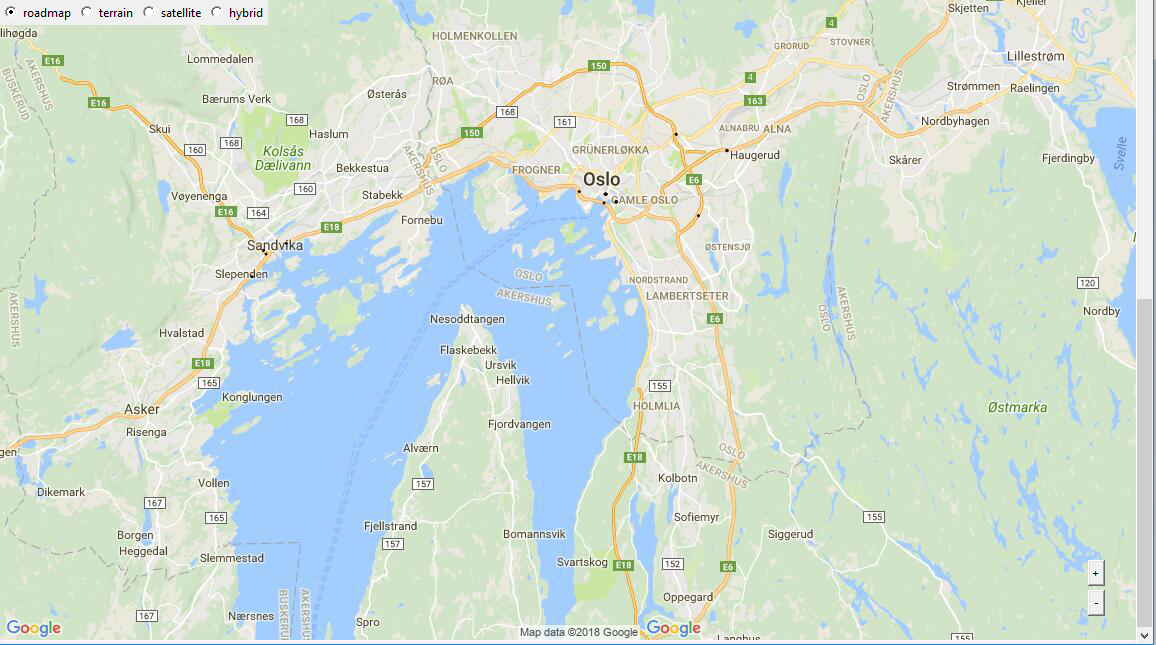
\includegraphics[width=12cm]{goompy}
\centering
\caption{A Goompy implementation of Google's static map API}
\label{fig:the_goompy}
\end{figure}

\newpage














\subsection{The Scrollbar}
Creating a functional scrollbar that responds to mouse dragging and mouse wheel events in Tkinter proved difficult, which is why Eugene Bakin's Tkinter scollable\cite{scrframe} frame was used. It is an open Github project. The file Frontend/scrframe.py contains his code with minor edits in order to be able to scroll with the mouse wheel, get the Tkinter focus, resetting scrollbar viewport and better resizing of the window. This module may also be run independently for testing purposes.




\subsection{NIPH dataframe}
The GUI module is structured in two parts: The buttons frame and the data frame, data frames visualise information from the backend. The NIPH data frame was created as it's own module to better organise code, the module serves as an easily implemented dataframe for the main program gui.py. The NIPH data frame was extended with the functionalities that allows for comparison of the NIPH data with all the other datasets at the different influenza seasons available. The frontend module NIPH\_frame.py was created to be implemented by the main file GUI.py and the file double\_y\_graphs.py provides the necessary supportive algorithms. Both files may be run individually for testing purposes. The comparison functions work in the way that the user selects a dataset to compare with by clicking a button in the top border. A drop-down menu will be produced giving the choices of cities and influenza seasons. Two graphs will then be drawn sharing the same x-axis but having different y-axes. This makes for easy comparison and querying the data in order to find possible correlations. While the graphs are loading a label displaying "Loading, please wait ..." will be shown in orange at the very right of the buttons panel. Figure \ref{fig:NIPH_compare} shows the NIPH comparing buttons panel.

\begin{figure}[ht]
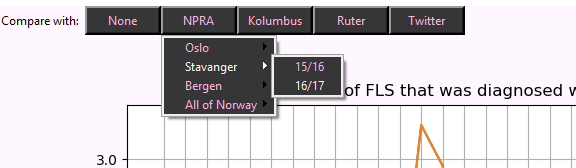
\includegraphics[width=16cm]{NIPH_compare}
\centering
\caption{NIPH comparing buttons panel}
\label{fig:NIPH_compare}
\end{figure}

\newpage

\subsection{NPRA dataframe}
In addition to the monthly and weekly datasets the hourly are presented in its own GUI module implemented by the main file GUI.py. The hourly datasets contains 58 different traffic registration stations from the cities of Bergen, Stavanger and Oslo and may be queried with the buttons-panel. The dropdown buttons provide the choices of hours to/from, weekdays to/from and months to/from from the years of 2013 to 2017 which can be selected from the checkbuttons, then there is a show button which initiates the query, lastly there is a save button which withdraws the data queried and saves it to a .csv file in a chosen directory.\\ The query may take up to a minute loading depending on how many years were selected, a label displaying "Loading, please wait ..." will be shown in orange to the very right of the query panel while the algorithms is running. If the query is invalid a label displaying "Error, invalid request!" will be shown in red at the same position. \\
On the left border a map is shown, displaying the available traffic registration stations in random colors and sizes (more about this in chapter 6). Figure \ref{fig:NPRA_query} shows the NPRA query buttons panel.

\begin{figure}[ht]
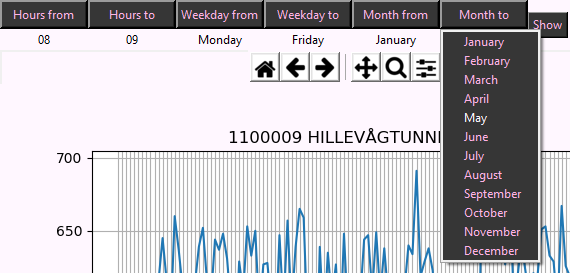
\includegraphics[width=16cm]{NPRA_query}
\centering
\caption{NPRA query buttons panel}
\label{fig:NPRA_query}
\end{figure}






\chapter{Results}
This chapter describes the subjective view of the results derived from this thesis's program detailed in chapter three and four. Discussion about the results is elaborated upon in the following chapter.



\section{NPRA}
There are three levels of data available: monthly, weekly and hourly. For this reason, the monthly dataset will be disregarded as there are better data available. Weekly data distinctly show the Norwegian holidays described in table \ref{table:jesus}. It is important to take these days into account when deriving information from these data, as otherwise, it would be easy to conclude wrongly. The most dramatic drop is the summer vacation, which luckily is outside the influenza season anyway. Another challenge with holidays and vacations is that the start and duration change yearly, and because of the Gregorian calendar set dates shift one day up the next weekday for the next year. This needs to be taken into consideration, and possibly weeded out or glossed over in order to avoid misinterpretations.

\begin{center}
\begin{table}[!h]
\begin{tabular}{ | m{9em} | m{10cm}| }
 \hline
 \textbf{Vacation/Holiday} & \textbf{When} \\ [0.5ex] 
 \hline
 Summer vacation & About nine weeks from the midth of June to the end of August  \\ 
 \hline 
 Autumn vacation & One week or a long weekend in September or October, usually in week 39, 40 or 41.\\ 
 \hline
 Christmas holiday & Usually two weeks from the end of December to the start of January\\ 
 \hline
 Winter vacation & usually in week 7, 8 or nine in February or March \\ 
  \hline
 Easter holiday & 10-11 days at the end of March or beginning of April \\ 
  \hline
 Other and Christian holy days & Labour Day, Ascension Day, Constitution Day \\ 
  \hline
\end{tabular}
\caption{The Norwegian holidays and vacations}
 \label{table:jesus}
\end{table}
\end{center}

Further, the weekly graphs show a considerable increase in traffic each year, when asked about this the NPRA admitted to their action plan to increase the numbers of traffic registration stations yearly. This increase of infrastructure is transparent in the graphs shown as jumps in the amount of traffic with each new year. From the end of November to the beginning of December there is a slight drop in the amount of traffic without there being any vacations or holidays, this anomaly might be correlated with the influenza season as numbers of reported virus observations and ILI incidents seems to increase at the same time. After influenza, occurrences spike and begin to decline traffic slightly return to normal over the course of January to June.
The weekly data is an aggregated set of many traffic registration stations based on the cities or the all of Norway, therefore roadworks, accidents or closed roads is not directly apparent. They are however visible, by assumption, on the hourly datasets as they only show one traffic registration station at a time. When in doubt of closed roads one could pick another traffic registration station nearby and see if it is also affected in the same manner. Another advantage with the hourly datasets is that there is not a dramatic yearly increase of traffic, which means more reliable data can be obtained, especially from the older traffic registration stations that have been operational for several years already. The map next to the hourly graph shows the available traffic registration stations to choose from.




\section{Twitter}
The way that twitter\_analyser.py works are that it simply counts the number of occurrences of tweets and then draws a graph based on that count. The Twitter data collected in twitter\_data.txt still contains duplicates although efforts were taken to prevent this. The duplicates may affect the graph drawn in batches as spikes where articles or hype are written about influenza or with other of the search terms. The Twitter data has a distinct pulse following the time when people post messages on social media the most by week\cite{socialTrend}, Mondays to Thursdays have a high yield of tweets, and then the weekends are calmer. This at least shows that the data collected is somewhat in accordance with other social media in other parts of the world. During the collection of tweets the event of the Norwegian Easter holiday occurred, from the graph shown the spikes even out and there is a more consistent flow of tweets throughout the holiday.
When comparing the datasets of twitter and NIPH there is a clear similarity between them. The Twitter data seems to follow the trend downwards with the NIPH when the season is coming close to an end. However, the Twitter data seems to be lagging behind by 10 weeks, even less so with the ILI data from Bergen. This is in direct contradiction with both research referenced earlier in chapter two, and with this thesis's expectations.





\section{Kolumbus}
The Kolumbus data is the least interesting as it does not have spatial specific data and that the data resolution is too low on a monthly basis to see any anomalies. The longer Norwegian vacations and holidays are still somewhat visible though. This goes to show that sufficient temporal resolution is critical in order to derive any useful information from data in this thesis.




\section{Ruter}
Comparing the Ruter data with the ILI data of Oslo is especially interesting because Ruter is the public transportation administrator in that city. As with the NPRA data the Norwegian holidays and vacations are apparent as described in section 5.1. The weeks of 47, 48 and 49 show a slight decrease of passenger travel without overlapping any vacations and holidays, there is also a slight increase of reported ILI every influenza season in those weeks. This correlation might be relevant and should be investigated further.
After the Christmas holiday passenger travel struggle for a few weeks to 'catch up' to a more stable level, interestingly enough the influenza seasons usually are on its peaks at that very time.
The amount of passenger travel also seems to be slightly increasing as the influenza season declines.

\chapter{Discussion}

In this chapter, the results and other constraints encountered will be discussed.

\section{Project Management}

Early in the planning and management phase of this thesis, it became evident that the Norwegian infrastructure for retrieving data from various public sources by API was not sufficient for the needs of this thesis. Therefore the initial plan to automate the collection of data needed was adapted to the means of acquiring the data by manually asking the various agencies and implementing their data hard-coded. This makes the program much less scalable and flexible than hoped for, and severely inhibits future contributions as it may be difficult to couple new data with the inputs of the backend's data structure. The missing automation part will probably hinder future use of this program. The only two APIs used are of American origin, namely Google static map and Twitter. In these regards the automation element that this thesis anticipated failed, however not by a critical means as manual retrieval of data was still possible.






\section{Project resolutions}
In the middle of the time scope for this thesis, a frontend to the backend was desired and thus planning to construct this began. There were several options for choosing not only from the languages the GUI would be based upon but consideration of how a map would be projected as well. These were the main concerns and had to be compatible with each other. The first choice was between Python's Tkinter GUI module and Node/Javascript GUI. The main reason Python was chosen was that it offered the easiest integration with the backend. Javascript prohibits direct reading from local files, and thus the backend would have to be mounted on a server in order to provide its functions to a frontend. The author of this thesis had little experience with this, and learning a whole new trade was daunting and seemed insurmountable within the rest time scope of this thesis, therefore the enticing of the familiarity of Python triumphed. In hindsight, it would probably be better to undertake a Node/Javascript approach because some sort of database to store the backend's data is needed anyway and is probably a more feasible solution, more on this in the following chapter.

Choosing a map implementation was difficult, Python has several options like GeoPandas, ipyleaflet, Google static map, cartopy, OpenStreetMap, and basemap. All of the mentioned was hard to install and was sorely limited in function and potential, except OpenStreetMap and Google static map. Upon further investigation Goompy, as described in chapter 2, was discovered and offered a nearly effortless implementation of the map in the already applied design of the frontend.

The advantage the Python solution has is that it requires few installations of external modules and is easily downloaded and mountable on many platforms.
The disadvantage with Python's module Matplotlib, which is used to draw graphs, is that drawing many graphs requires a lot of memory and processor resources, therefore it is important to manage the graphs drawn, and only load those that need be loaded at a time, flushing those that are no longer in use.
The advantage of Google static map is that it is a well implemented and established service with consistent qualitative measures. Google offers fewer road details than OpenStreetMap, and that serves this thesis perfectly as the visualization needed was simply showing locations of traffic registration stations and not necessarily other roads.
The disadvantages with Google static map is that there are standard usage limits (which can simply be overcome with paying for more). Pixel resolution is set to a maximum of 640x640 pixels, and the free usage is limited to 25.000 map loads per 24 hours. These two limits are not really a problem: The pixel limit is overcome by simply requesting more map loads and then combining those to create as big a picture as desired, and the map loads limit is very high. On average Goompy does 4 map loads per zoom (thus creating a big map of 1280x1280 pixels) and 25.000 / 4 = 6250 zooms per 24 hours, average Norwegian working hours per day is 7.5 hours, this means that one would reach the limit if there are 6.250 / 7.5 / 60 = 13.9 zooms per second. This limit was never reached in testing and although it is a high limit if reached the map simply stops working for the remainder of the time to the next 24 hours. Perhaps the most severe limit Google static map have for the scope of this thesis is its maximum URL size of 8192 characters. Figure \ref{fig:google_url} show the programs URL that it sends to the Google map servers, containing a standard map and fifty-three traffic registration stations each with their individually different sizes and colors this surmounts to a total of 4.975 characters already, which is 60.7\% of the total allowed. 

\begin{figure}[h]
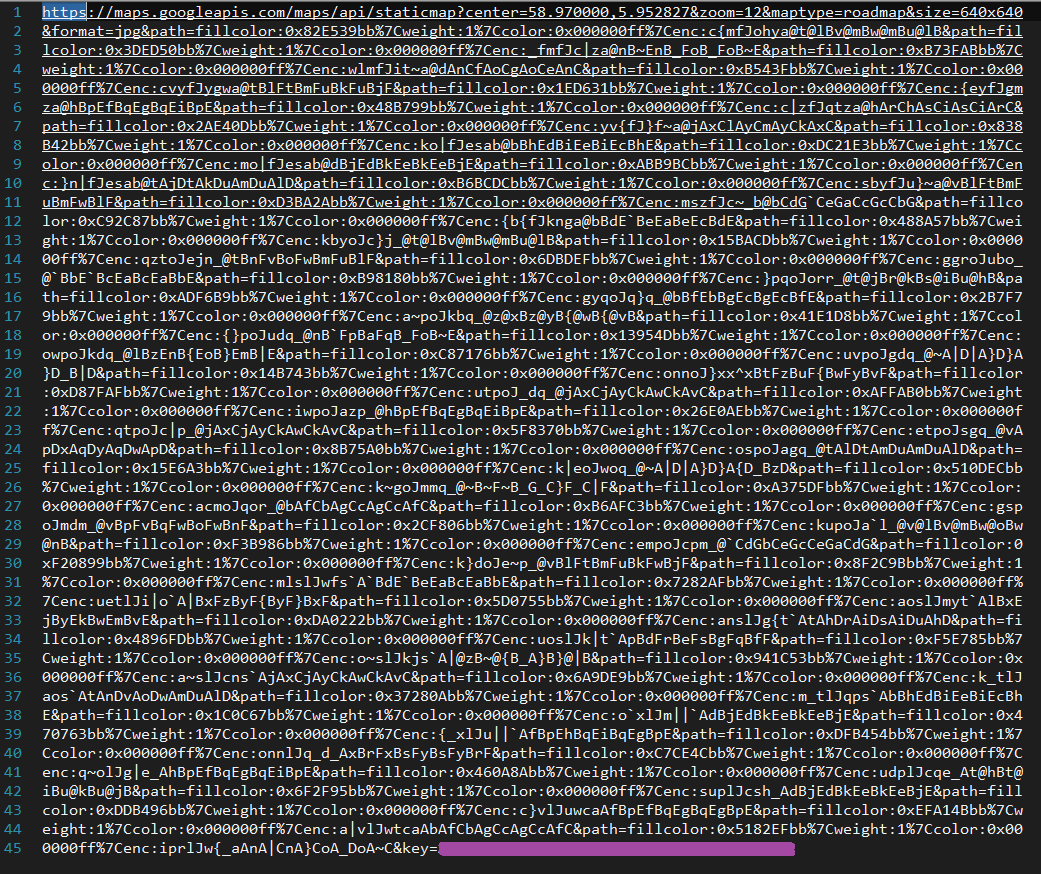
\includegraphics[width=12cm]{Google_static_map_URL}
\centering
\caption{Size of the programs Google static map URLs}
\label{fig:google_url}
\end{figure}

Although the url have encoded polylines, which compresses the data, it is already quite long, Loading all of Norway's current 10.066 traffic registration stations using Google static map with this thesis's current algorithms is not feasible, although this could be solved by clustering the traffic registration stations together, and only loading what you actually can see on the map. This would require more Goompy modifications by somehow fetching only those traffic registration stations that are actually currently visible on the map.
The program would still be considered modular and scalable with the chosen technologies and implemented algorithms, although better solutions may be applied. Further discussion of possible future works is described in the following chapter

\chapter{Conclusion}
This thesis presents a program that is a prototype of what an automated collection of multi-source spatial information for emergency management systems may look like. It contains a basic assembly of the system and describes the various components of the program. The program visualises collected data both spatially on a map and by traditional graphs. The information is presented by category and contains multiple tools to help with investigative analysis. Tools like moving, zooming in and out on graph assets, capturing graph state, adjusting subplot parameters, comparison of graphs, querying graphs and map visualisation. The system is modular and scalable and allows for the addition of further features, as well as an integration of new data sources from other agencies.\\

The early months of this thesis's time scope were characterized by collecting data from various agencies to be used in the backend. This was notably a tough grind, as getting access to data would take several weeks followed by multiple rounds of communication back and forth, with reminders and careful explanations along the way. The cooperation with the involved agents varied in quality, but the overall service was sufficient. This process involved some waiting days with modest development; this is a common occurrence in professional work.\\

Automated collection of multi-source spatial information is a critical component of a real-time societal indicator surveillance system, as such systems are dependent on access to large amounts of data from a variety of sources. The automation part may not become practical for years to come, as the general Norwegian public API infrastructure is not sufficiently implemented at the current point in time. Implementing more relevant sources should also be a priority, as well as collecting spatial data for specific regions of Norway. Big Data acquisition and analysis efforts must be coordinated with further research on method development, to integrate the methods into the next generation of flu surveillance systems. Combining information from multiple sources provides a powerful capability to assist in emergency management, and efforts to additionally support data collection of citizen behaviour on a macro scale should be encouraged.







\appendix
\chapter{Appendix Title}

%\printbibliography
\bibliography{references}
\bibliographystyle{ieeetr}
%\usepackage{url}

\end{document}